\documentclass[twoside]{book}

% Packages required by doxygen
\usepackage{fixltx2e}
\usepackage{calc}
\usepackage{doxygen}
\usepackage[export]{adjustbox} % also loads graphicx
\usepackage{graphicx}
\usepackage[utf8]{inputenc}
\usepackage{makeidx}
\usepackage{multicol}
\usepackage{multirow}
\PassOptionsToPackage{warn}{textcomp}
\usepackage{textcomp}
\usepackage[nointegrals]{wasysym}
\usepackage[table]{xcolor}

% Font selection
\usepackage[T1]{fontenc}
\usepackage[scaled=.90]{helvet}
\usepackage{courier}
\usepackage{amssymb}
\usepackage{sectsty}
\renewcommand{\familydefault}{\sfdefault}
\allsectionsfont{%
  \fontseries{bc}\selectfont%
  \color{darkgray}%
}
\renewcommand{\DoxyLabelFont}{%
  \fontseries{bc}\selectfont%
  \color{darkgray}%
}
\newcommand{\+}{\discretionary{\mbox{\scriptsize$\hookleftarrow$}}{}{}}

% Page & text layout
\usepackage{geometry}
\geometry{%
  a4paper,%
  top=2.5cm,%
  bottom=2.5cm,%
  left=2.5cm,%
  right=2.5cm%
}
\tolerance=750
\hfuzz=15pt
\hbadness=750
\setlength{\emergencystretch}{15pt}
\setlength{\parindent}{0cm}
\setlength{\parskip}{3ex plus 2ex minus 2ex}
\makeatletter
\renewcommand{\paragraph}{%
  \@startsection{paragraph}{4}{0ex}{-1.0ex}{1.0ex}{%
    \normalfont\normalsize\bfseries\SS@parafont%
  }%
}
\renewcommand{\subparagraph}{%
  \@startsection{subparagraph}{5}{0ex}{-1.0ex}{1.0ex}{%
    \normalfont\normalsize\bfseries\SS@subparafont%
  }%
}
\makeatother

% Headers & footers
\usepackage{fancyhdr}
\pagestyle{fancyplain}
\fancyhead[LE]{\fancyplain{}{\bfseries\thepage}}
\fancyhead[CE]{\fancyplain{}{}}
\fancyhead[RE]{\fancyplain{}{\bfseries\leftmark}}
\fancyhead[LO]{\fancyplain{}{\bfseries\rightmark}}
\fancyhead[CO]{\fancyplain{}{}}
\fancyhead[RO]{\fancyplain{}{\bfseries\thepage}}
\fancyfoot[LE]{\fancyplain{}{}}
\fancyfoot[CE]{\fancyplain{}{}}
\fancyfoot[RE]{\fancyplain{}{\bfseries\scriptsize Generated by Doxygen }}
\fancyfoot[LO]{\fancyplain{}{\bfseries\scriptsize Generated by Doxygen }}
\fancyfoot[CO]{\fancyplain{}{}}
\fancyfoot[RO]{\fancyplain{}{}}
\renewcommand{\footrulewidth}{0.4pt}
\renewcommand{\chaptermark}[1]{%
  \markboth{#1}{}%
}
\renewcommand{\sectionmark}[1]{%
  \markright{\thesection\ #1}%
}

% Indices & bibliography
\usepackage{natbib}
\usepackage[titles]{tocloft}
\setcounter{tocdepth}{3}
\setcounter{secnumdepth}{5}
\makeindex

% Hyperlinks (required, but should be loaded last)
\usepackage{ifpdf}
\ifpdf
  \usepackage[pdftex,pagebackref=true]{hyperref}
\else
  \usepackage[ps2pdf,pagebackref=true]{hyperref}
\fi
\hypersetup{%
  colorlinks=true,%
  linkcolor=blue,%
  citecolor=blue,%
  unicode%
}

% Custom commands
\newcommand{\clearemptydoublepage}{%
  \newpage{\pagestyle{empty}\cleardoublepage}%
}

\usepackage{caption}
\captionsetup{labelsep=space,justification=centering,font={bf},singlelinecheck=off,skip=4pt,position=top}

%===== C O N T E N T S =====

\begin{document}

% Titlepage & ToC
\hypersetup{pageanchor=false,
             bookmarksnumbered=true,
             pdfencoding=unicode
            }
\pagenumbering{roman}
\begin{titlepage}
\vspace*{7cm}
\begin{center}%
{\Large Authentication Authorization Manager }\\
\vspace*{1cm}
{\large Generated by Doxygen 1.8.11}\\
\end{center}
\end{titlepage}
\clearemptydoublepage
\tableofcontents
\clearemptydoublepage
\pagenumbering{arabic}
\hypersetup{pageanchor=true}

%--- Begin generated contents ---
\chapter{R\+E\+A\+D\+ME}
\label{md_README}
\hypertarget{md_README}{}
\href{https://api.travis-ci.org/symbiote-h2020/AuthenticationAuthorizationManager}{\tt } \href{https://codecov.io/github/symbiote-h2020/AuthenticationAuthorizationManager}{\tt }

\section*{Authentication\+Authorization\+Manager}
\chapter{Hierarchical Index}
\section{Class Hierarchy}
This inheritance list is sorted roughly, but not completely, alphabetically\+:\begin{DoxyCompactList}
\item \contentsline{section}{eu.\+h2020.\+symbiote.\+security.\+rest.\+Application\+Registration\+Controller}{\pageref{classeu_1_1h2020_1_1symbiote_1_1security_1_1rest_1_1ApplicationRegistrationController}}{}
\item \contentsline{section}{eu.\+h2020.\+symbiote.\+security.\+Authentication\+Authorization\+Manager}{\pageref{classeu_1_1h2020_1_1symbiote_1_1security_1_1AuthenticationAuthorizationManager}}{}
\item \contentsline{section}{eu.\+h2020.\+symbiote.\+security.\+rest.\+Error\+Controller}{\pageref{classeu_1_1h2020_1_1symbiote_1_1security_1_1rest_1_1ErrorController}}{}
\item Filter\begin{DoxyCompactList}
\item \contentsline{section}{eu.\+h2020.\+symbiote.\+security.\+commons.\+filters.\+C\+O\+R\+S\+Filter}{\pageref{classeu_1_1h2020_1_1symbiote_1_1security_1_1commons_1_1filters_1_1CORSFilter}}{}
\end{DoxyCompactList}
\item \contentsline{section}{eu.\+h2020.\+symbiote.\+security.\+rest.\+Login\+Controller}{\pageref{classeu_1_1h2020_1_1symbiote_1_1security_1_1rest_1_1LoginController}}{}
\item \contentsline{section}{eu.\+h2020.\+symbiote.\+security.\+services.\+Login\+Service}{\pageref{classeu_1_1h2020_1_1symbiote_1_1security_1_1services_1_1LoginService}}{}
\item \contentsline{section}{eu.\+h2020.\+symbiote.\+security.\+rest.\+Other\+Controller}{\pageref{classeu_1_1h2020_1_1symbiote_1_1security_1_1rest_1_1OtherController}}{}
\item \contentsline{section}{eu.\+h2020.\+symbiote.\+security.\+commons.\+Platform}{\pageref{classeu_1_1h2020_1_1symbiote_1_1security_1_1commons_1_1Platform}}{}
\item \contentsline{section}{eu.\+h2020.\+symbiote.\+security.\+services.\+Platform\+Registration\+Service}{\pageref{classeu_1_1h2020_1_1symbiote_1_1security_1_1services_1_1PlatformRegistrationService}}{}
\item \contentsline{section}{eu.\+h2020.\+symbiote.\+security.\+amqp.\+Rabbit\+Manager}{\pageref{classeu_1_1h2020_1_1symbiote_1_1security_1_1amqp_1_1RabbitManager}}{}
\item \contentsline{section}{eu.\+h2020.\+symbiote.\+security.\+commons.\+Registration\+Manager}{\pageref{classeu_1_1h2020_1_1symbiote_1_1security_1_1commons_1_1RegistrationManager}}{}
\item \contentsline{section}{eu.\+h2020.\+symbiote.\+security.\+rest.\+Token\+Controller}{\pageref{classeu_1_1h2020_1_1symbiote_1_1security_1_1rest_1_1TokenController}}{}
\item \contentsline{section}{eu.\+h2020.\+symbiote.\+security.\+commons.\+Token\+Manager}{\pageref{classeu_1_1h2020_1_1symbiote_1_1security_1_1commons_1_1TokenManager}}{}
\item \contentsline{section}{eu.\+h2020.\+symbiote.\+security.\+services.\+Token\+Service}{\pageref{classeu_1_1h2020_1_1symbiote_1_1security_1_1services_1_1TokenService}}{}
\item \contentsline{section}{eu.\+h2020.\+symbiote.\+security.\+commons.\+User}{\pageref{classeu_1_1h2020_1_1symbiote_1_1security_1_1commons_1_1User}}{}
\item \contentsline{section}{eu.\+h2020.\+symbiote.\+security.\+services.\+User\+Registration\+Service}{\pageref{classeu_1_1h2020_1_1symbiote_1_1security_1_1services_1_1UserRegistrationService}}{}
\item \contentsline{section}{eu.\+h2020.\+symbiote.\+security.\+commons.\+Virtual\+File}{\pageref{classeu_1_1h2020_1_1symbiote_1_1security_1_1commons_1_1VirtualFile}}{}
\item \contentsline{section}{eu.\+h2020.\+symbiote.\+security.\+services.\+Zip\+Service}{\pageref{classeu_1_1h2020_1_1symbiote_1_1security_1_1services_1_1ZipService}}{}
\item Default\+Consumer\begin{DoxyCompactList}
\item \contentsline{section}{eu.\+h2020.\+symbiote.\+security.\+amqp.\+consumers.\+Application\+Registration\+Request\+Consumer\+Service}{\pageref{classeu_1_1h2020_1_1symbiote_1_1security_1_1amqp_1_1consumers_1_1ApplicationRegistrationRequestConsumerService}}{}
\item \contentsline{section}{eu.\+h2020.\+symbiote.\+security.\+amqp.\+consumers.\+Check\+Token\+Revocation\+Request\+Consumer\+Service}{\pageref{classeu_1_1h2020_1_1symbiote_1_1security_1_1amqp_1_1consumers_1_1CheckTokenRevocationRequestConsumerService}}{}
\item \contentsline{section}{eu.\+h2020.\+symbiote.\+security.\+amqp.\+consumers.\+Login\+Request\+Consumer\+Service}{\pageref{classeu_1_1h2020_1_1symbiote_1_1security_1_1amqp_1_1consumers_1_1LoginRequestConsumerService}}{}
\item \contentsline{section}{eu.\+h2020.\+symbiote.\+security.\+amqp.\+consumers.\+Owned\+Platform\+Details\+Request\+Consumer\+Service}{\pageref{classeu_1_1h2020_1_1symbiote_1_1security_1_1amqp_1_1consumers_1_1OwnedPlatformDetailsRequestConsumerService}}{}
\item \contentsline{section}{eu.\+h2020.\+symbiote.\+security.\+amqp.\+consumers.\+Platform\+Registration\+Request\+Consumer\+Service}{\pageref{classeu_1_1h2020_1_1symbiote_1_1security_1_1amqp_1_1consumers_1_1PlatformRegistrationRequestConsumerService}}{}
\end{DoxyCompactList}
\item Mongo\+Repository\begin{DoxyCompactList}
\item \contentsline{section}{eu.\+h2020.\+symbiote.\+security.\+repositories.\+Platform\+Repository}{\pageref{interfaceeu_1_1h2020_1_1symbiote_1_1security_1_1repositories_1_1PlatformRepository}}{}
\item \contentsline{section}{eu.\+h2020.\+symbiote.\+security.\+repositories.\+Revoked\+Certificates\+Repository}{\pageref{interfaceeu_1_1h2020_1_1symbiote_1_1security_1_1repositories_1_1RevokedCertificatesRepository}}{}
\item \contentsline{section}{eu.\+h2020.\+symbiote.\+security.\+repositories.\+Token\+Repository}{\pageref{interfaceeu_1_1h2020_1_1symbiote_1_1security_1_1repositories_1_1TokenRepository}}{}
\item \contentsline{section}{eu.\+h2020.\+symbiote.\+security.\+repositories.\+User\+Repository}{\pageref{interfaceeu_1_1h2020_1_1symbiote_1_1security_1_1repositories_1_1UserRepository}}{}
\end{DoxyCompactList}
\end{DoxyCompactList}

\chapter{Class Index}
\section{Class List}
Here are the classes, structs, unions and interfaces with brief descriptions\+:\begin{DoxyCompactList}
\item\contentsline{section}{\hyperlink{classeu_1_1h2020_1_1symbiote_1_1security_1_1rest_1_1ApplicationRegistrationController}{eu.\+h2020.\+symbiote.\+security.\+rest.\+Application\+Registration\+Controller} }{\pageref{classeu_1_1h2020_1_1symbiote_1_1security_1_1rest_1_1ApplicationRegistrationController}}{}
\item\contentsline{section}{\hyperlink{classeu_1_1h2020_1_1symbiote_1_1security_1_1amqp_1_1consumers_1_1ApplicationRegistrationRequestConsumerService}{eu.\+h2020.\+symbiote.\+security.\+amqp.\+consumers.\+Application\+Registration\+Request\+Consumer\+Service} }{\pageref{classeu_1_1h2020_1_1symbiote_1_1security_1_1amqp_1_1consumers_1_1ApplicationRegistrationRequestConsumerService}}{}
\item\contentsline{section}{\hyperlink{classeu_1_1h2020_1_1symbiote_1_1security_1_1AuthenticationAuthorizationManager}{eu.\+h2020.\+symbiote.\+security.\+Authentication\+Authorization\+Manager} }{\pageref{classeu_1_1h2020_1_1symbiote_1_1security_1_1AuthenticationAuthorizationManager}}{}
\item\contentsline{section}{\hyperlink{classeu_1_1h2020_1_1symbiote_1_1security_1_1amqp_1_1consumers_1_1CheckTokenRevocationRequestConsumerService}{eu.\+h2020.\+symbiote.\+security.\+amqp.\+consumers.\+Check\+Token\+Revocation\+Request\+Consumer\+Service} }{\pageref{classeu_1_1h2020_1_1symbiote_1_1security_1_1amqp_1_1consumers_1_1CheckTokenRevocationRequestConsumerService}}{}
\item\contentsline{section}{\hyperlink{classeu_1_1h2020_1_1symbiote_1_1security_1_1commons_1_1filters_1_1CORSFilter}{eu.\+h2020.\+symbiote.\+security.\+commons.\+filters.\+C\+O\+R\+S\+Filter} }{\pageref{classeu_1_1h2020_1_1symbiote_1_1security_1_1commons_1_1filters_1_1CORSFilter}}{}
\item\contentsline{section}{\hyperlink{classeu_1_1h2020_1_1symbiote_1_1security_1_1rest_1_1ErrorController}{eu.\+h2020.\+symbiote.\+security.\+rest.\+Error\+Controller} }{\pageref{classeu_1_1h2020_1_1symbiote_1_1security_1_1rest_1_1ErrorController}}{}
\item\contentsline{section}{\hyperlink{classeu_1_1h2020_1_1symbiote_1_1security_1_1rest_1_1LoginController}{eu.\+h2020.\+symbiote.\+security.\+rest.\+Login\+Controller} }{\pageref{classeu_1_1h2020_1_1symbiote_1_1security_1_1rest_1_1LoginController}}{}
\item\contentsline{section}{\hyperlink{classeu_1_1h2020_1_1symbiote_1_1security_1_1amqp_1_1consumers_1_1LoginRequestConsumerService}{eu.\+h2020.\+symbiote.\+security.\+amqp.\+consumers.\+Login\+Request\+Consumer\+Service} }{\pageref{classeu_1_1h2020_1_1symbiote_1_1security_1_1amqp_1_1consumers_1_1LoginRequestConsumerService}}{}
\item\contentsline{section}{\hyperlink{classeu_1_1h2020_1_1symbiote_1_1security_1_1services_1_1LoginService}{eu.\+h2020.\+symbiote.\+security.\+services.\+Login\+Service} }{\pageref{classeu_1_1h2020_1_1symbiote_1_1security_1_1services_1_1LoginService}}{}
\item\contentsline{section}{\hyperlink{classeu_1_1h2020_1_1symbiote_1_1security_1_1rest_1_1OtherController}{eu.\+h2020.\+symbiote.\+security.\+rest.\+Other\+Controller} }{\pageref{classeu_1_1h2020_1_1symbiote_1_1security_1_1rest_1_1OtherController}}{}
\item\contentsline{section}{\hyperlink{classeu_1_1h2020_1_1symbiote_1_1security_1_1amqp_1_1consumers_1_1OwnedPlatformDetailsRequestConsumerService}{eu.\+h2020.\+symbiote.\+security.\+amqp.\+consumers.\+Owned\+Platform\+Details\+Request\+Consumer\+Service} }{\pageref{classeu_1_1h2020_1_1symbiote_1_1security_1_1amqp_1_1consumers_1_1OwnedPlatformDetailsRequestConsumerService}}{}
\item\contentsline{section}{\hyperlink{classeu_1_1h2020_1_1symbiote_1_1security_1_1commons_1_1Platform}{eu.\+h2020.\+symbiote.\+security.\+commons.\+Platform} }{\pageref{classeu_1_1h2020_1_1symbiote_1_1security_1_1commons_1_1Platform}}{}
\item\contentsline{section}{\hyperlink{classeu_1_1h2020_1_1symbiote_1_1security_1_1amqp_1_1consumers_1_1PlatformRegistrationRequestConsumerService}{eu.\+h2020.\+symbiote.\+security.\+amqp.\+consumers.\+Platform\+Registration\+Request\+Consumer\+Service} }{\pageref{classeu_1_1h2020_1_1symbiote_1_1security_1_1amqp_1_1consumers_1_1PlatformRegistrationRequestConsumerService}}{}
\item\contentsline{section}{\hyperlink{classeu_1_1h2020_1_1symbiote_1_1security_1_1services_1_1PlatformRegistrationService}{eu.\+h2020.\+symbiote.\+security.\+services.\+Platform\+Registration\+Service} }{\pageref{classeu_1_1h2020_1_1symbiote_1_1security_1_1services_1_1PlatformRegistrationService}}{}
\item\contentsline{section}{\hyperlink{interfaceeu_1_1h2020_1_1symbiote_1_1security_1_1repositories_1_1PlatformRepository}{eu.\+h2020.\+symbiote.\+security.\+repositories.\+Platform\+Repository} }{\pageref{interfaceeu_1_1h2020_1_1symbiote_1_1security_1_1repositories_1_1PlatformRepository}}{}
\item\contentsline{section}{\hyperlink{classeu_1_1h2020_1_1symbiote_1_1security_1_1amqp_1_1RabbitManager}{eu.\+h2020.\+symbiote.\+security.\+amqp.\+Rabbit\+Manager} }{\pageref{classeu_1_1h2020_1_1symbiote_1_1security_1_1amqp_1_1RabbitManager}}{}
\item\contentsline{section}{\hyperlink{classeu_1_1h2020_1_1symbiote_1_1security_1_1commons_1_1RegistrationManager}{eu.\+h2020.\+symbiote.\+security.\+commons.\+Registration\+Manager} }{\pageref{classeu_1_1h2020_1_1symbiote_1_1security_1_1commons_1_1RegistrationManager}}{}
\item\contentsline{section}{\hyperlink{interfaceeu_1_1h2020_1_1symbiote_1_1security_1_1repositories_1_1RevokedCertificatesRepository}{eu.\+h2020.\+symbiote.\+security.\+repositories.\+Revoked\+Certificates\+Repository} }{\pageref{interfaceeu_1_1h2020_1_1symbiote_1_1security_1_1repositories_1_1RevokedCertificatesRepository}}{}
\item\contentsline{section}{\hyperlink{classeu_1_1h2020_1_1symbiote_1_1security_1_1rest_1_1TokenController}{eu.\+h2020.\+symbiote.\+security.\+rest.\+Token\+Controller} }{\pageref{classeu_1_1h2020_1_1symbiote_1_1security_1_1rest_1_1TokenController}}{}
\item\contentsline{section}{\hyperlink{classeu_1_1h2020_1_1symbiote_1_1security_1_1commons_1_1TokenManager}{eu.\+h2020.\+symbiote.\+security.\+commons.\+Token\+Manager} }{\pageref{classeu_1_1h2020_1_1symbiote_1_1security_1_1commons_1_1TokenManager}}{}
\item\contentsline{section}{\hyperlink{interfaceeu_1_1h2020_1_1symbiote_1_1security_1_1repositories_1_1TokenRepository}{eu.\+h2020.\+symbiote.\+security.\+repositories.\+Token\+Repository} }{\pageref{interfaceeu_1_1h2020_1_1symbiote_1_1security_1_1repositories_1_1TokenRepository}}{}
\item\contentsline{section}{\hyperlink{classeu_1_1h2020_1_1symbiote_1_1security_1_1services_1_1TokenService}{eu.\+h2020.\+symbiote.\+security.\+services.\+Token\+Service} }{\pageref{classeu_1_1h2020_1_1symbiote_1_1security_1_1services_1_1TokenService}}{}
\item\contentsline{section}{\hyperlink{classeu_1_1h2020_1_1symbiote_1_1security_1_1commons_1_1User}{eu.\+h2020.\+symbiote.\+security.\+commons.\+User} }{\pageref{classeu_1_1h2020_1_1symbiote_1_1security_1_1commons_1_1User}}{}
\item\contentsline{section}{\hyperlink{classeu_1_1h2020_1_1symbiote_1_1security_1_1services_1_1UserRegistrationService}{eu.\+h2020.\+symbiote.\+security.\+services.\+User\+Registration\+Service} }{\pageref{classeu_1_1h2020_1_1symbiote_1_1security_1_1services_1_1UserRegistrationService}}{}
\item\contentsline{section}{\hyperlink{interfaceeu_1_1h2020_1_1symbiote_1_1security_1_1repositories_1_1UserRepository}{eu.\+h2020.\+symbiote.\+security.\+repositories.\+User\+Repository} }{\pageref{interfaceeu_1_1h2020_1_1symbiote_1_1security_1_1repositories_1_1UserRepository}}{}
\item\contentsline{section}{\hyperlink{classeu_1_1h2020_1_1symbiote_1_1security_1_1commons_1_1VirtualFile}{eu.\+h2020.\+symbiote.\+security.\+commons.\+Virtual\+File} }{\pageref{classeu_1_1h2020_1_1symbiote_1_1security_1_1commons_1_1VirtualFile}}{}
\item\contentsline{section}{\hyperlink{classeu_1_1h2020_1_1symbiote_1_1security_1_1services_1_1ZipService}{eu.\+h2020.\+symbiote.\+security.\+services.\+Zip\+Service} }{\pageref{classeu_1_1h2020_1_1symbiote_1_1security_1_1services_1_1ZipService}}{}
\end{DoxyCompactList}

\chapter{Class Documentation}
\hypertarget{classeu_1_1h2020_1_1symbiote_1_1security_1_1rest_1_1ApplicationRegistrationController}{}\section{eu.\+h2020.\+symbiote.\+security.\+rest.\+Application\+Registration\+Controller Class Reference}
\label{classeu_1_1h2020_1_1symbiote_1_1security_1_1rest_1_1ApplicationRegistrationController}\index{eu.\+h2020.\+symbiote.\+security.\+rest.\+Application\+Registration\+Controller@{eu.\+h2020.\+symbiote.\+security.\+rest.\+Application\+Registration\+Controller}}


Collaboration diagram for eu.\+h2020.\+symbiote.\+security.\+rest.\+Application\+Registration\+Controller\+:
\nopagebreak
\begin{figure}[H]
\begin{center}
\leavevmode
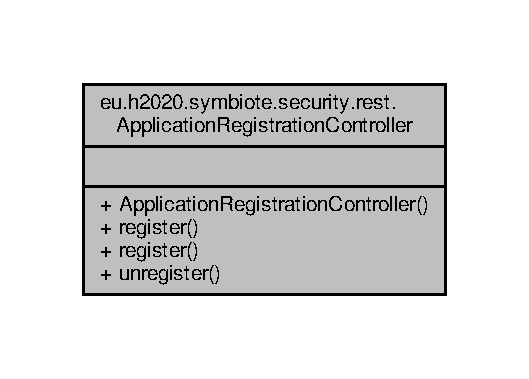
\includegraphics[width=254pt]{classeu_1_1h2020_1_1symbiote_1_1security_1_1rest_1_1ApplicationRegistrationController__coll__graph}
\end{center}
\end{figure}
\subsection*{Public Member Functions}
\begin{DoxyCompactItemize}
\item 
{\bfseries Application\+Registration\+Controller} (\hyperlink{classeu_1_1h2020_1_1symbiote_1_1security_1_1services_1_1UserRegistrationService}{User\+Registration\+Service} registration\+Service, \hyperlink{classeu_1_1h2020_1_1symbiote_1_1security_1_1services_1_1ZipService}{Zip\+Service} zip\+Service)\hypertarget{classeu_1_1h2020_1_1symbiote_1_1security_1_1rest_1_1ApplicationRegistrationController_a499ce6f5c03029ba9748ce8d3724c189}{}\label{classeu_1_1h2020_1_1symbiote_1_1security_1_1rest_1_1ApplicationRegistrationController_a499ce6f5c03029ba9748ce8d3724c189}

\item 
Response\+Entity$<$?$>$ {\bfseries register} (@Request\+Param Map$<$ String, String $>$ request\+Map, Http\+Servlet\+Response response)  throws A\+A\+M\+Exception, I\+O\+Exception, Zip\+Exception \hypertarget{classeu_1_1h2020_1_1symbiote_1_1security_1_1rest_1_1ApplicationRegistrationController_abf530fcf7f2895473187a79480acd949}{}\label{classeu_1_1h2020_1_1symbiote_1_1security_1_1rest_1_1ApplicationRegistrationController_abf530fcf7f2895473187a79480acd949}

\item 
Response\+Entity$<$?$>$ {\bfseries register} (@Request\+Body User\+Registration\+Request request)\hypertarget{classeu_1_1h2020_1_1symbiote_1_1security_1_1rest_1_1ApplicationRegistrationController_a5a1352f84bd849039cdde117e929ddda}{}\label{classeu_1_1h2020_1_1symbiote_1_1security_1_1rest_1_1ApplicationRegistrationController_a5a1352f84bd849039cdde117e929ddda}

\item 
Response\+Entity$<$?$>$ {\bfseries unregister} (@Request\+Body User\+Registration\+Request request)\hypertarget{classeu_1_1h2020_1_1symbiote_1_1security_1_1rest_1_1ApplicationRegistrationController_aa410f10874546858272e474b5baf5076}{}\label{classeu_1_1h2020_1_1symbiote_1_1security_1_1rest_1_1ApplicationRegistrationController_aa410f10874546858272e474b5baf5076}

\end{DoxyCompactItemize}


\subsection{Detailed Description}
Spring controller to handle H\+T\+T\+PS requests related to the R\+E\+S\+Tful web service associated to user/app registration service in Cloud A\+AM component.

\begin{DoxyAuthor}{Author}
Daniele Caldarola (C\+N\+IT) 

Nemanja Ignjatov (U\+N\+I\+V\+IE) 
\end{DoxyAuthor}
\begin{DoxySeeAlso}{See also}
Login\+Service 
\end{DoxySeeAlso}


The documentation for this class was generated from the following file\+:\begin{DoxyCompactItemize}
\item 
src/main/java/eu/h2020/symbiote/security/rest/Application\+Registration\+Controller.\+java\end{DoxyCompactItemize}

\hypertarget{classeu_1_1h2020_1_1symbiote_1_1security_1_1amqp_1_1consumers_1_1ApplicationRegistrationRequestConsumerService}{}\section{eu.\+h2020.\+symbiote.\+security.\+amqp.\+consumers.\+Application\+Registration\+Request\+Consumer\+Service Class Reference}
\label{classeu_1_1h2020_1_1symbiote_1_1security_1_1amqp_1_1consumers_1_1ApplicationRegistrationRequestConsumerService}\index{eu.\+h2020.\+symbiote.\+security.\+amqp.\+consumers.\+Application\+Registration\+Request\+Consumer\+Service@{eu.\+h2020.\+symbiote.\+security.\+amqp.\+consumers.\+Application\+Registration\+Request\+Consumer\+Service}}


Inheritance diagram for eu.\+h2020.\+symbiote.\+security.\+amqp.\+consumers.\+Application\+Registration\+Request\+Consumer\+Service\+:
\nopagebreak
\begin{figure}[H]
\begin{center}
\leavevmode
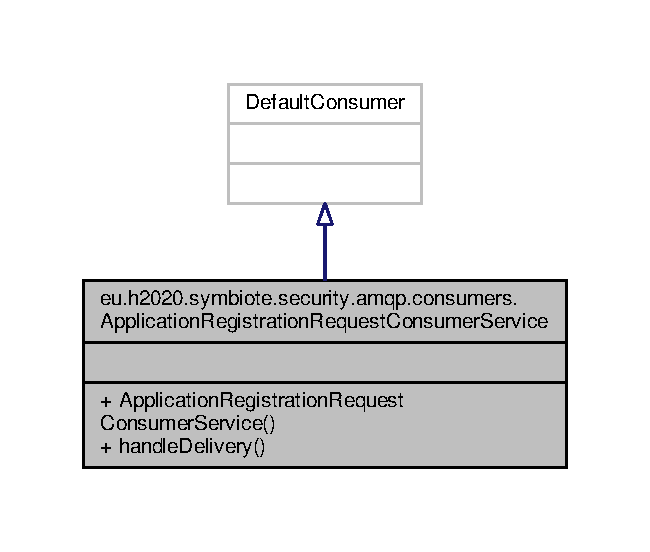
\includegraphics[width=312pt]{classeu_1_1h2020_1_1symbiote_1_1security_1_1amqp_1_1consumers_1_1ApplicationRegistrationRequestConsumerService__inherit__graph}
\end{center}
\end{figure}


Collaboration diagram for eu.\+h2020.\+symbiote.\+security.\+amqp.\+consumers.\+Application\+Registration\+Request\+Consumer\+Service\+:
\nopagebreak
\begin{figure}[H]
\begin{center}
\leavevmode
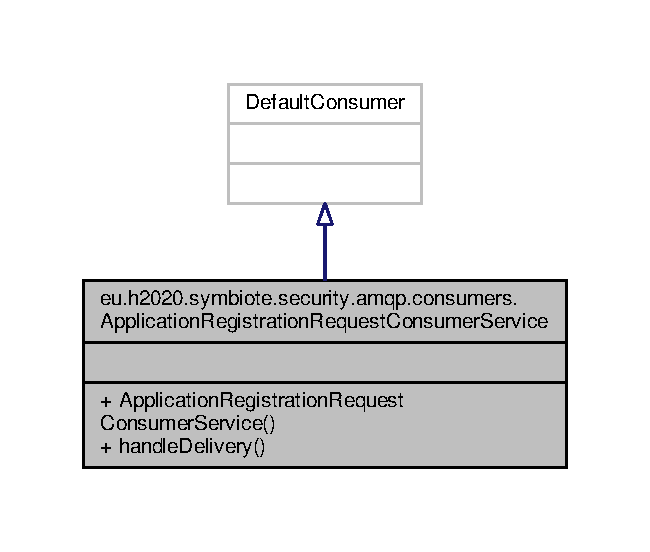
\includegraphics[width=312pt]{classeu_1_1h2020_1_1symbiote_1_1security_1_1amqp_1_1consumers_1_1ApplicationRegistrationRequestConsumerService__coll__graph}
\end{center}
\end{figure}
\subsection*{Public Member Functions}
\begin{DoxyCompactItemize}
\item 
\hyperlink{classeu_1_1h2020_1_1symbiote_1_1security_1_1amqp_1_1consumers_1_1ApplicationRegistrationRequestConsumerService_a33e736ed17c521abd360c3f99878f867}{Application\+Registration\+Request\+Consumer\+Service} (Channel channel, \hyperlink{classeu_1_1h2020_1_1symbiote_1_1security_1_1services_1_1UserRegistrationService}{User\+Registration\+Service} user\+Registration\+Service)
\item 
void \hyperlink{classeu_1_1h2020_1_1symbiote_1_1security_1_1amqp_1_1consumers_1_1ApplicationRegistrationRequestConsumerService_a9a0833ca543b20f7686a6d45b4f2ea88}{handle\+Delivery} (String consumer\+Tag, Envelope envelope, A\+M\+Q\+P.\+Basic\+Properties properties, byte\mbox{[}$\,$\mbox{]} body)  throws I\+O\+Exception 
\end{DoxyCompactItemize}


\subsection{Detailed Description}
Rabbit\+MQ Consumer implementation used for Applications\textquotesingle{} Registration actions

\begin{DoxyAuthor}{Author}
Mikołaj Dobski (P\+S\+NC) 
\end{DoxyAuthor}


\subsection{Constructor \& Destructor Documentation}
\index{eu\+::h2020\+::symbiote\+::security\+::amqp\+::consumers\+::\+Application\+Registration\+Request\+Consumer\+Service@{eu\+::h2020\+::symbiote\+::security\+::amqp\+::consumers\+::\+Application\+Registration\+Request\+Consumer\+Service}!Application\+Registration\+Request\+Consumer\+Service@{Application\+Registration\+Request\+Consumer\+Service}}
\index{Application\+Registration\+Request\+Consumer\+Service@{Application\+Registration\+Request\+Consumer\+Service}!eu\+::h2020\+::symbiote\+::security\+::amqp\+::consumers\+::\+Application\+Registration\+Request\+Consumer\+Service@{eu\+::h2020\+::symbiote\+::security\+::amqp\+::consumers\+::\+Application\+Registration\+Request\+Consumer\+Service}}
\subsubsection[{\texorpdfstring{Application\+Registration\+Request\+Consumer\+Service(\+Channel channel, User\+Registration\+Service user\+Registration\+Service)}{ApplicationRegistrationRequestConsumerService(Channel channel, UserRegistrationService userRegistrationService)}}]{\setlength{\rightskip}{0pt plus 5cm}eu.\+h2020.\+symbiote.\+security.\+amqp.\+consumers.\+Application\+Registration\+Request\+Consumer\+Service.\+Application\+Registration\+Request\+Consumer\+Service (
\begin{DoxyParamCaption}
\item[{Channel}]{channel, }
\item[{{\bf User\+Registration\+Service}}]{user\+Registration\+Service}
\end{DoxyParamCaption}
)}\hypertarget{classeu_1_1h2020_1_1symbiote_1_1security_1_1amqp_1_1consumers_1_1ApplicationRegistrationRequestConsumerService_a33e736ed17c521abd360c3f99878f867}{}\label{classeu_1_1h2020_1_1symbiote_1_1security_1_1amqp_1_1consumers_1_1ApplicationRegistrationRequestConsumerService_a33e736ed17c521abd360c3f99878f867}
Constructs a new instance and records its association to the passed-\/in channel. Managers beans passed as parameters because of lack of possibility to inject it to consumer.


\begin{DoxyParams}{Parameters}
{\em channel} & the channel to which this consumer is attached \\
\hline
\end{DoxyParams}


\subsection{Member Function Documentation}
\index{eu\+::h2020\+::symbiote\+::security\+::amqp\+::consumers\+::\+Application\+Registration\+Request\+Consumer\+Service@{eu\+::h2020\+::symbiote\+::security\+::amqp\+::consumers\+::\+Application\+Registration\+Request\+Consumer\+Service}!handle\+Delivery@{handle\+Delivery}}
\index{handle\+Delivery@{handle\+Delivery}!eu\+::h2020\+::symbiote\+::security\+::amqp\+::consumers\+::\+Application\+Registration\+Request\+Consumer\+Service@{eu\+::h2020\+::symbiote\+::security\+::amqp\+::consumers\+::\+Application\+Registration\+Request\+Consumer\+Service}}
\subsubsection[{\texorpdfstring{handle\+Delivery(\+String consumer\+Tag, Envelope envelope, A\+M\+Q\+P.\+Basic\+Properties properties, byte[] body)}{handleDelivery(String consumerTag, Envelope envelope, AMQP.BasicProperties properties, byte[] body)}}]{\setlength{\rightskip}{0pt plus 5cm}void eu.\+h2020.\+symbiote.\+security.\+amqp.\+consumers.\+Application\+Registration\+Request\+Consumer\+Service.\+handle\+Delivery (
\begin{DoxyParamCaption}
\item[{String}]{consumer\+Tag, }
\item[{Envelope}]{envelope, }
\item[{A\+M\+Q\+P.\+Basic\+Properties}]{properties, }
\item[{byte\mbox{[}$\,$\mbox{]}}]{body}
\end{DoxyParamCaption}
) throws I\+O\+Exception}\hypertarget{classeu_1_1h2020_1_1symbiote_1_1security_1_1amqp_1_1consumers_1_1ApplicationRegistrationRequestConsumerService_a9a0833ca543b20f7686a6d45b4f2ea88}{}\label{classeu_1_1h2020_1_1symbiote_1_1security_1_1amqp_1_1consumers_1_1ApplicationRegistrationRequestConsumerService_a9a0833ca543b20f7686a6d45b4f2ea88}
Called when a {\ttfamily {\bfseries basic.\+deliver}} is received for this consumer.


\begin{DoxyParams}{Parameters}
{\em consumer\+Tag} & the {\itshape consumer tag} associated with the consumer \\
\hline
{\em envelope} & packaging data for the message \\
\hline
{\em properties} & content header data for the message \\
\hline
{\em body} & the message body (opaque, client-\/specific byte array) \\
\hline
\end{DoxyParams}

\begin{DoxyExceptions}{Exceptions}
{\em I\+O\+Exception} & if the consumer encounters an I/O error while processing the message \\
\hline
\end{DoxyExceptions}
\begin{DoxySeeAlso}{See also}
Envelope 
\end{DoxySeeAlso}


The documentation for this class was generated from the following file\+:\begin{DoxyCompactItemize}
\item 
src/main/java/eu/h2020/symbiote/security/amqp/consumers/Application\+Registration\+Request\+Consumer\+Service.\+java\end{DoxyCompactItemize}

\hypertarget{classeu_1_1h2020_1_1symbiote_1_1security_1_1AuthenticationAuthorizationManager}{}\section{eu.\+h2020.\+symbiote.\+security.\+Authentication\+Authorization\+Manager Class Reference}
\label{classeu_1_1h2020_1_1symbiote_1_1security_1_1AuthenticationAuthorizationManager}\index{eu.\+h2020.\+symbiote.\+security.\+Authentication\+Authorization\+Manager@{eu.\+h2020.\+symbiote.\+security.\+Authentication\+Authorization\+Manager}}


Collaboration diagram for eu.\+h2020.\+symbiote.\+security.\+Authentication\+Authorization\+Manager\+:
\nopagebreak
\begin{figure}[H]
\begin{center}
\leavevmode
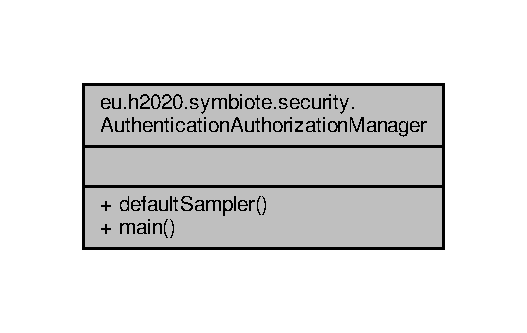
\includegraphics[width=253pt]{classeu_1_1h2020_1_1symbiote_1_1security_1_1AuthenticationAuthorizationManager__coll__graph}
\end{center}
\end{figure}
\subsection*{Classes}
\begin{DoxyCompactItemize}
\item 
class {\bfseries C\+LR}
\end{DoxyCompactItemize}
\subsection*{Public Member Functions}
\begin{DoxyCompactItemize}
\item 
Always\+Sampler {\bfseries default\+Sampler} ()\hypertarget{classeu_1_1h2020_1_1symbiote_1_1security_1_1AuthenticationAuthorizationManager_a36a9f29e75344a484082ac9e4fed677c}{}\label{classeu_1_1h2020_1_1symbiote_1_1security_1_1AuthenticationAuthorizationManager_a36a9f29e75344a484082ac9e4fed677c}

\end{DoxyCompactItemize}
\subsection*{Static Public Member Functions}
\begin{DoxyCompactItemize}
\item 
static void {\bfseries main} (String\mbox{[}$\,$\mbox{]} args)\hypertarget{classeu_1_1h2020_1_1symbiote_1_1security_1_1AuthenticationAuthorizationManager_a2fc88f9c6ed7f8a92e718d96b56443c0}{}\label{classeu_1_1h2020_1_1symbiote_1_1security_1_1AuthenticationAuthorizationManager_a2fc88f9c6ed7f8a92e718d96b56443c0}

\end{DoxyCompactItemize}


\subsection{Detailed Description}
Spring Boot Application class for \hyperlink{classeu_1_1h2020_1_1symbiote_1_1security_1_1AuthenticationAuthorizationManager}{Authentication\+Authorization\+Manager} (A\+AM) component.

\begin{DoxyAuthor}{Author}
Daniele Caldarola (C\+N\+IT) 

Nemanja Ignjatov (U\+N\+I\+V\+IE) 

Mikolaj Dobski (P\+S\+NC) 
\end{DoxyAuthor}


The documentation for this class was generated from the following file\+:\begin{DoxyCompactItemize}
\item 
src/main/java/eu/h2020/symbiote/security/Authentication\+Authorization\+Manager.\+java\end{DoxyCompactItemize}

\hypertarget{classeu_1_1h2020_1_1symbiote_1_1security_1_1amqp_1_1consumers_1_1CheckTokenRevocationRequestConsumerService}{}\section{eu.\+h2020.\+symbiote.\+security.\+amqp.\+consumers.\+Check\+Token\+Revocation\+Request\+Consumer\+Service Class Reference}
\label{classeu_1_1h2020_1_1symbiote_1_1security_1_1amqp_1_1consumers_1_1CheckTokenRevocationRequestConsumerService}\index{eu.\+h2020.\+symbiote.\+security.\+amqp.\+consumers.\+Check\+Token\+Revocation\+Request\+Consumer\+Service@{eu.\+h2020.\+symbiote.\+security.\+amqp.\+consumers.\+Check\+Token\+Revocation\+Request\+Consumer\+Service}}


Inheritance diagram for eu.\+h2020.\+symbiote.\+security.\+amqp.\+consumers.\+Check\+Token\+Revocation\+Request\+Consumer\+Service\+:
\nopagebreak
\begin{figure}[H]
\begin{center}
\leavevmode
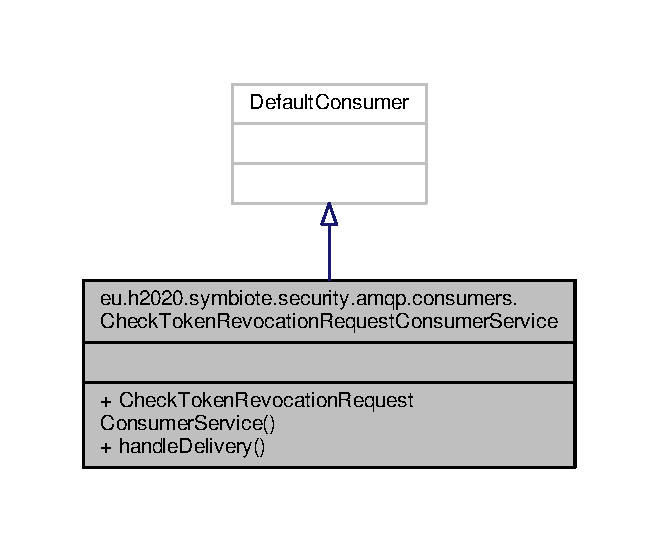
\includegraphics[width=316pt]{classeu_1_1h2020_1_1symbiote_1_1security_1_1amqp_1_1consumers_1_1CheckTokenRevocationRequestConsumerService__inherit__graph}
\end{center}
\end{figure}


Collaboration diagram for eu.\+h2020.\+symbiote.\+security.\+amqp.\+consumers.\+Check\+Token\+Revocation\+Request\+Consumer\+Service\+:
\nopagebreak
\begin{figure}[H]
\begin{center}
\leavevmode
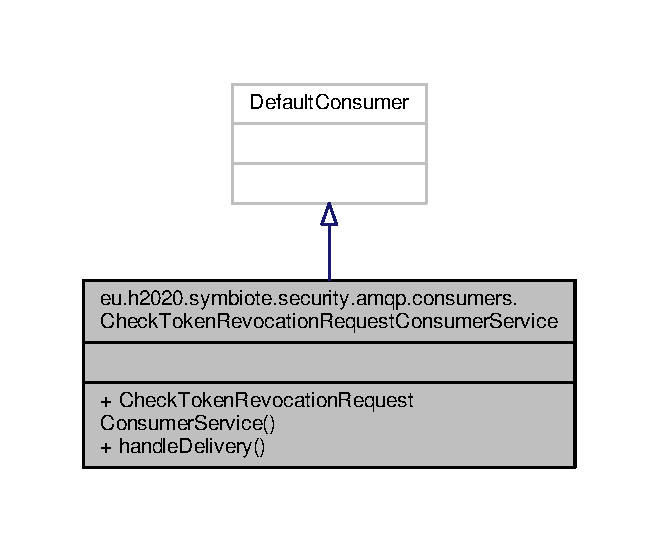
\includegraphics[width=316pt]{classeu_1_1h2020_1_1symbiote_1_1security_1_1amqp_1_1consumers_1_1CheckTokenRevocationRequestConsumerService__coll__graph}
\end{center}
\end{figure}
\subsection*{Public Member Functions}
\begin{DoxyCompactItemize}
\item 
\hyperlink{classeu_1_1h2020_1_1symbiote_1_1security_1_1amqp_1_1consumers_1_1CheckTokenRevocationRequestConsumerService_af94d46927f2be0bb40d3c514ea75ede1}{Check\+Token\+Revocation\+Request\+Consumer\+Service} (Channel channel, \hyperlink{classeu_1_1h2020_1_1symbiote_1_1security_1_1services_1_1TokenService}{Token\+Service} token\+Service)
\item 
void \hyperlink{classeu_1_1h2020_1_1symbiote_1_1security_1_1amqp_1_1consumers_1_1CheckTokenRevocationRequestConsumerService_a99b366f93335c08c6de1aa2a77d967e0}{handle\+Delivery} (String consumer\+Tag, Envelope envelope, A\+M\+Q\+P.\+Basic\+Properties properties, byte\mbox{[}$\,$\mbox{]} body)  throws I\+O\+Exception 
\end{DoxyCompactItemize}


\subsection{Detailed Description}
Rabbit\+MQ Consumer implementation used for token revocation checking actions 

\subsection{Constructor \& Destructor Documentation}
\index{eu\+::h2020\+::symbiote\+::security\+::amqp\+::consumers\+::\+Check\+Token\+Revocation\+Request\+Consumer\+Service@{eu\+::h2020\+::symbiote\+::security\+::amqp\+::consumers\+::\+Check\+Token\+Revocation\+Request\+Consumer\+Service}!Check\+Token\+Revocation\+Request\+Consumer\+Service@{Check\+Token\+Revocation\+Request\+Consumer\+Service}}
\index{Check\+Token\+Revocation\+Request\+Consumer\+Service@{Check\+Token\+Revocation\+Request\+Consumer\+Service}!eu\+::h2020\+::symbiote\+::security\+::amqp\+::consumers\+::\+Check\+Token\+Revocation\+Request\+Consumer\+Service@{eu\+::h2020\+::symbiote\+::security\+::amqp\+::consumers\+::\+Check\+Token\+Revocation\+Request\+Consumer\+Service}}
\subsubsection[{\texorpdfstring{Check\+Token\+Revocation\+Request\+Consumer\+Service(\+Channel channel, Token\+Service token\+Service)}{CheckTokenRevocationRequestConsumerService(Channel channel, TokenService tokenService)}}]{\setlength{\rightskip}{0pt plus 5cm}eu.\+h2020.\+symbiote.\+security.\+amqp.\+consumers.\+Check\+Token\+Revocation\+Request\+Consumer\+Service.\+Check\+Token\+Revocation\+Request\+Consumer\+Service (
\begin{DoxyParamCaption}
\item[{Channel}]{channel, }
\item[{{\bf Token\+Service}}]{token\+Service}
\end{DoxyParamCaption}
)}\hypertarget{classeu_1_1h2020_1_1symbiote_1_1security_1_1amqp_1_1consumers_1_1CheckTokenRevocationRequestConsumerService_af94d46927f2be0bb40d3c514ea75ede1}{}\label{classeu_1_1h2020_1_1symbiote_1_1security_1_1amqp_1_1consumers_1_1CheckTokenRevocationRequestConsumerService_af94d46927f2be0bb40d3c514ea75ede1}
Constructs a new instance and records its association to the passed-\/in channel. Managers beans passed as parameters because of lack of possibility to inject it to consumer.


\begin{DoxyParams}{Parameters}
{\em channel} & the channel to which this consumer is attached \\
\hline
\end{DoxyParams}


\subsection{Member Function Documentation}
\index{eu\+::h2020\+::symbiote\+::security\+::amqp\+::consumers\+::\+Check\+Token\+Revocation\+Request\+Consumer\+Service@{eu\+::h2020\+::symbiote\+::security\+::amqp\+::consumers\+::\+Check\+Token\+Revocation\+Request\+Consumer\+Service}!handle\+Delivery@{handle\+Delivery}}
\index{handle\+Delivery@{handle\+Delivery}!eu\+::h2020\+::symbiote\+::security\+::amqp\+::consumers\+::\+Check\+Token\+Revocation\+Request\+Consumer\+Service@{eu\+::h2020\+::symbiote\+::security\+::amqp\+::consumers\+::\+Check\+Token\+Revocation\+Request\+Consumer\+Service}}
\subsubsection[{\texorpdfstring{handle\+Delivery(\+String consumer\+Tag, Envelope envelope, A\+M\+Q\+P.\+Basic\+Properties properties, byte[] body)}{handleDelivery(String consumerTag, Envelope envelope, AMQP.BasicProperties properties, byte[] body)}}]{\setlength{\rightskip}{0pt plus 5cm}void eu.\+h2020.\+symbiote.\+security.\+amqp.\+consumers.\+Check\+Token\+Revocation\+Request\+Consumer\+Service.\+handle\+Delivery (
\begin{DoxyParamCaption}
\item[{String}]{consumer\+Tag, }
\item[{Envelope}]{envelope, }
\item[{A\+M\+Q\+P.\+Basic\+Properties}]{properties, }
\item[{byte\mbox{[}$\,$\mbox{]}}]{body}
\end{DoxyParamCaption}
) throws I\+O\+Exception}\hypertarget{classeu_1_1h2020_1_1symbiote_1_1security_1_1amqp_1_1consumers_1_1CheckTokenRevocationRequestConsumerService_a99b366f93335c08c6de1aa2a77d967e0}{}\label{classeu_1_1h2020_1_1symbiote_1_1security_1_1amqp_1_1consumers_1_1CheckTokenRevocationRequestConsumerService_a99b366f93335c08c6de1aa2a77d967e0}
Called when a {\ttfamily {\bfseries basic.\+deliver}} is received for this consumer.


\begin{DoxyParams}{Parameters}
{\em consumer\+Tag} & the {\itshape consumer tag} associated with the consumer \\
\hline
{\em envelope} & packaging data for the message \\
\hline
{\em properties} & content header data for the message \\
\hline
{\em body} & the message body (opaque, client-\/specific byte array) \\
\hline
\end{DoxyParams}

\begin{DoxyExceptions}{Exceptions}
{\em I\+O\+Exception} & if the consumer encounters an I/O error while processing the message \\
\hline
\end{DoxyExceptions}
\begin{DoxySeeAlso}{See also}
Envelope 
\end{DoxySeeAlso}


The documentation for this class was generated from the following file\+:\begin{DoxyCompactItemize}
\item 
src/main/java/eu/h2020/symbiote/security/amqp/consumers/Check\+Token\+Revocation\+Request\+Consumer\+Service.\+java\end{DoxyCompactItemize}

\hypertarget{classeu_1_1h2020_1_1symbiote_1_1security_1_1commons_1_1filters_1_1CORSFilter}{}\section{eu.\+h2020.\+symbiote.\+security.\+commons.\+filters.\+C\+O\+R\+S\+Filter Class Reference}
\label{classeu_1_1h2020_1_1symbiote_1_1security_1_1commons_1_1filters_1_1CORSFilter}\index{eu.\+h2020.\+symbiote.\+security.\+commons.\+filters.\+C\+O\+R\+S\+Filter@{eu.\+h2020.\+symbiote.\+security.\+commons.\+filters.\+C\+O\+R\+S\+Filter}}


Inheritance diagram for eu.\+h2020.\+symbiote.\+security.\+commons.\+filters.\+C\+O\+R\+S\+Filter\+:
\nopagebreak
\begin{figure}[H]
\begin{center}
\leavevmode
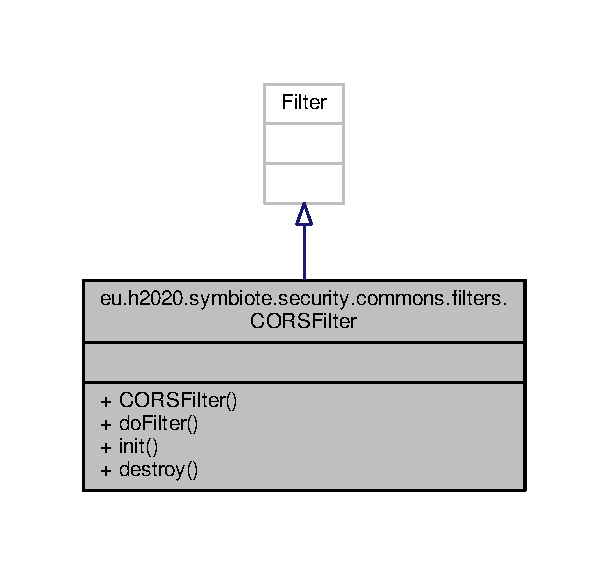
\includegraphics[width=292pt]{classeu_1_1h2020_1_1symbiote_1_1security_1_1commons_1_1filters_1_1CORSFilter__inherit__graph}
\end{center}
\end{figure}


Collaboration diagram for eu.\+h2020.\+symbiote.\+security.\+commons.\+filters.\+C\+O\+R\+S\+Filter\+:
\nopagebreak
\begin{figure}[H]
\begin{center}
\leavevmode
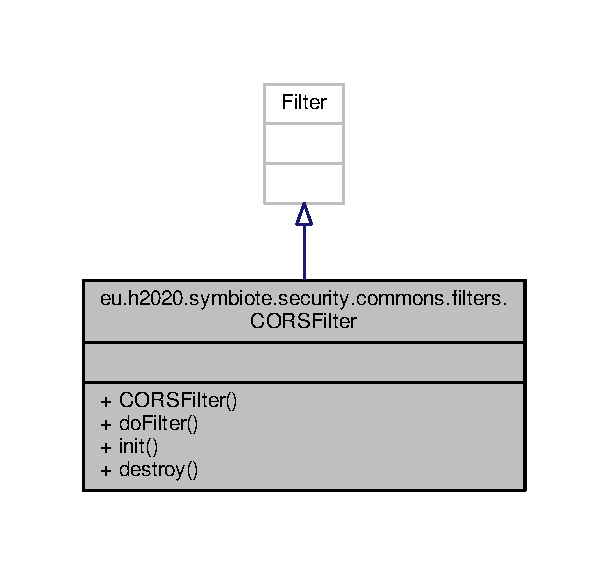
\includegraphics[width=292pt]{classeu_1_1h2020_1_1symbiote_1_1security_1_1commons_1_1filters_1_1CORSFilter__coll__graph}
\end{center}
\end{figure}
\subsection*{Public Member Functions}
\begin{DoxyCompactItemize}
\item 
void {\bfseries do\+Filter} (Servlet\+Request req, Servlet\+Response res, Filter\+Chain chain)  throws I\+O\+Exception, Servlet\+Exception \hypertarget{classeu_1_1h2020_1_1symbiote_1_1security_1_1commons_1_1filters_1_1CORSFilter_acc7cf17f670b1190ba0331899938c05e}{}\label{classeu_1_1h2020_1_1symbiote_1_1security_1_1commons_1_1filters_1_1CORSFilter_acc7cf17f670b1190ba0331899938c05e}

\item 
void {\bfseries init} (Filter\+Config filter\+Config)\hypertarget{classeu_1_1h2020_1_1symbiote_1_1security_1_1commons_1_1filters_1_1CORSFilter_ae2c300d63712bcb26e3a3f8fc07795e5}{}\label{classeu_1_1h2020_1_1symbiote_1_1security_1_1commons_1_1filters_1_1CORSFilter_ae2c300d63712bcb26e3a3f8fc07795e5}

\item 
void {\bfseries destroy} ()\hypertarget{classeu_1_1h2020_1_1symbiote_1_1security_1_1commons_1_1filters_1_1CORSFilter_aca378a9022997b996a9b886a5a4d549f}{}\label{classeu_1_1h2020_1_1symbiote_1_1security_1_1commons_1_1filters_1_1CORSFilter_aca378a9022997b996a9b886a5a4d549f}

\end{DoxyCompactItemize}


The documentation for this class was generated from the following file\+:\begin{DoxyCompactItemize}
\item 
src/main/java/eu/h2020/symbiote/security/commons/filters/C\+O\+R\+S\+Filter.\+java\end{DoxyCompactItemize}

\hypertarget{classeu_1_1h2020_1_1symbiote_1_1security_1_1rest_1_1ErrorController}{}\section{eu.\+h2020.\+symbiote.\+security.\+rest.\+Error\+Controller Class Reference}
\label{classeu_1_1h2020_1_1symbiote_1_1security_1_1rest_1_1ErrorController}\index{eu.\+h2020.\+symbiote.\+security.\+rest.\+Error\+Controller@{eu.\+h2020.\+symbiote.\+security.\+rest.\+Error\+Controller}}


Collaboration diagram for eu.\+h2020.\+symbiote.\+security.\+rest.\+Error\+Controller\+:
\nopagebreak
\begin{figure}[H]
\begin{center}
\leavevmode
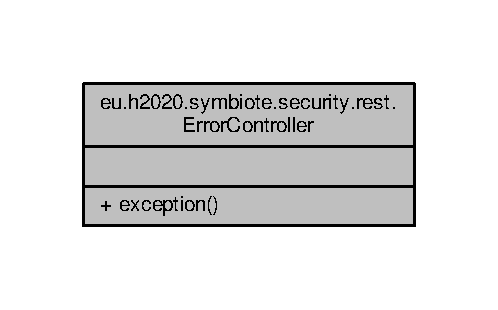
\includegraphics[width=239pt]{classeu_1_1h2020_1_1symbiote_1_1security_1_1rest_1_1ErrorController__coll__graph}
\end{center}
\end{figure}
\subsection*{Public Member Functions}
\begin{DoxyCompactItemize}
\item 
String {\bfseries exception} (final Throwable throwable, final Model model)\hypertarget{classeu_1_1h2020_1_1symbiote_1_1security_1_1rest_1_1ErrorController_a47948914af52f1fb02563de2ac3bcb48}{}\label{classeu_1_1h2020_1_1symbiote_1_1security_1_1rest_1_1ErrorController_a47948914af52f1fb02563de2ac3bcb48}

\end{DoxyCompactItemize}


The documentation for this class was generated from the following file\+:\begin{DoxyCompactItemize}
\item 
src/main/java/eu/h2020/symbiote/security/rest/Error\+Controller.\+java\end{DoxyCompactItemize}

\hypertarget{classeu_1_1h2020_1_1symbiote_1_1security_1_1rest_1_1LoginController}{}\section{eu.\+h2020.\+symbiote.\+security.\+rest.\+Login\+Controller Class Reference}
\label{classeu_1_1h2020_1_1symbiote_1_1security_1_1rest_1_1LoginController}\index{eu.\+h2020.\+symbiote.\+security.\+rest.\+Login\+Controller@{eu.\+h2020.\+symbiote.\+security.\+rest.\+Login\+Controller}}


Collaboration diagram for eu.\+h2020.\+symbiote.\+security.\+rest.\+Login\+Controller\+:
\nopagebreak
\begin{figure}[H]
\begin{center}
\leavevmode
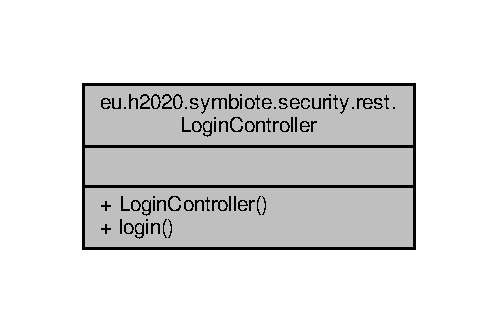
\includegraphics[width=239pt]{classeu_1_1h2020_1_1symbiote_1_1security_1_1rest_1_1LoginController__coll__graph}
\end{center}
\end{figure}
\subsection*{Public Member Functions}
\begin{DoxyCompactItemize}
\item 
{\bfseries Login\+Controller} (\hyperlink{classeu_1_1h2020_1_1symbiote_1_1security_1_1services_1_1LoginService}{Login\+Service} login\+Service)\hypertarget{classeu_1_1h2020_1_1symbiote_1_1security_1_1rest_1_1LoginController_a2f04e63185380098756b5ae1012794f3}{}\label{classeu_1_1h2020_1_1symbiote_1_1security_1_1rest_1_1LoginController_a2f04e63185380098756b5ae1012794f3}

\item 
Response\+Entity$<$?$>$ {\bfseries login} (@Request\+Body Credentials user)\hypertarget{classeu_1_1h2020_1_1symbiote_1_1security_1_1rest_1_1LoginController_a305fadbc421654617487035743d13d1c}{}\label{classeu_1_1h2020_1_1symbiote_1_1security_1_1rest_1_1LoginController_a305fadbc421654617487035743d13d1c}

\end{DoxyCompactItemize}


\subsection{Detailed Description}
Spring controller to handle H\+T\+T\+PS requests related to the R\+E\+S\+Tful web service associated to user/app login service in Cloud A\+AM component.

\begin{DoxyAuthor}{Author}
Daniele Caldarola (C\+N\+IT) 

Nemanja Ignjatov (U\+N\+I\+V\+IE) 
\end{DoxyAuthor}
\begin{DoxySeeAlso}{See also}
Login\+Service 
\end{DoxySeeAlso}


The documentation for this class was generated from the following file\+:\begin{DoxyCompactItemize}
\item 
src/main/java/eu/h2020/symbiote/security/rest/Login\+Controller.\+java\end{DoxyCompactItemize}

\hypertarget{classeu_1_1h2020_1_1symbiote_1_1security_1_1amqp_1_1consumers_1_1LoginRequestConsumerService}{}\section{eu.\+h2020.\+symbiote.\+security.\+amqp.\+consumers.\+Login\+Request\+Consumer\+Service Class Reference}
\label{classeu_1_1h2020_1_1symbiote_1_1security_1_1amqp_1_1consumers_1_1LoginRequestConsumerService}\index{eu.\+h2020.\+symbiote.\+security.\+amqp.\+consumers.\+Login\+Request\+Consumer\+Service@{eu.\+h2020.\+symbiote.\+security.\+amqp.\+consumers.\+Login\+Request\+Consumer\+Service}}


Inheritance diagram for eu.\+h2020.\+symbiote.\+security.\+amqp.\+consumers.\+Login\+Request\+Consumer\+Service\+:
\nopagebreak
\begin{figure}[H]
\begin{center}
\leavevmode
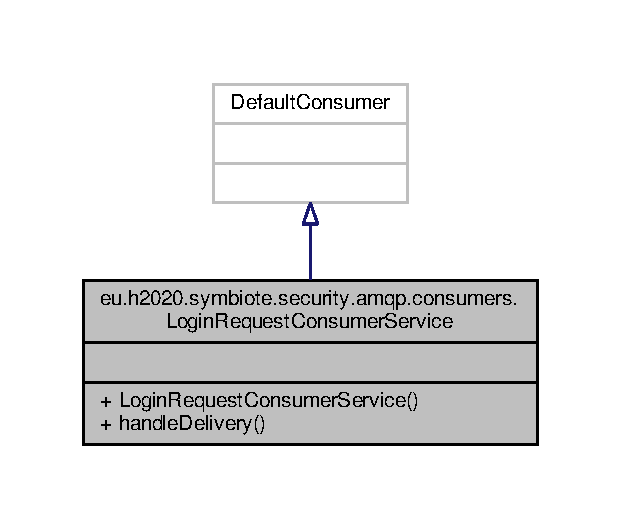
\includegraphics[width=298pt]{classeu_1_1h2020_1_1symbiote_1_1security_1_1amqp_1_1consumers_1_1LoginRequestConsumerService__inherit__graph}
\end{center}
\end{figure}


Collaboration diagram for eu.\+h2020.\+symbiote.\+security.\+amqp.\+consumers.\+Login\+Request\+Consumer\+Service\+:
\nopagebreak
\begin{figure}[H]
\begin{center}
\leavevmode
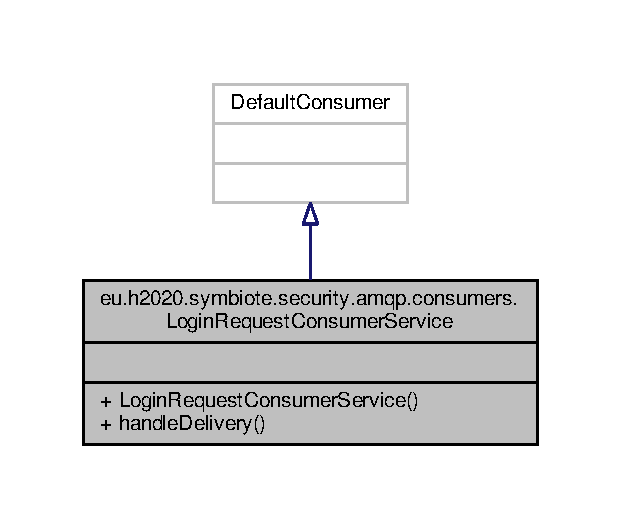
\includegraphics[width=298pt]{classeu_1_1h2020_1_1symbiote_1_1security_1_1amqp_1_1consumers_1_1LoginRequestConsumerService__coll__graph}
\end{center}
\end{figure}
\subsection*{Public Member Functions}
\begin{DoxyCompactItemize}
\item 
\hyperlink{classeu_1_1h2020_1_1symbiote_1_1security_1_1amqp_1_1consumers_1_1LoginRequestConsumerService_a69c09badb0af0855ec3c07caa8306458}{Login\+Request\+Consumer\+Service} (Channel channel, \hyperlink{classeu_1_1h2020_1_1symbiote_1_1security_1_1services_1_1LoginService}{Login\+Service} login\+Service)
\item 
void \hyperlink{classeu_1_1h2020_1_1symbiote_1_1security_1_1amqp_1_1consumers_1_1LoginRequestConsumerService_af09972ec03b30e58f3e4f6cd85011e6e}{handle\+Delivery} (String consumer\+Tag, Envelope envelope, A\+M\+Q\+P.\+Basic\+Properties properties, byte\mbox{[}$\,$\mbox{]} body)  throws I\+O\+Exception 
\end{DoxyCompactItemize}


\subsection{Detailed Description}
Rabbit\+MQ Consumer implementation used for Login actions 

\subsection{Constructor \& Destructor Documentation}
\index{eu\+::h2020\+::symbiote\+::security\+::amqp\+::consumers\+::\+Login\+Request\+Consumer\+Service@{eu\+::h2020\+::symbiote\+::security\+::amqp\+::consumers\+::\+Login\+Request\+Consumer\+Service}!Login\+Request\+Consumer\+Service@{Login\+Request\+Consumer\+Service}}
\index{Login\+Request\+Consumer\+Service@{Login\+Request\+Consumer\+Service}!eu\+::h2020\+::symbiote\+::security\+::amqp\+::consumers\+::\+Login\+Request\+Consumer\+Service@{eu\+::h2020\+::symbiote\+::security\+::amqp\+::consumers\+::\+Login\+Request\+Consumer\+Service}}
\subsubsection[{\texorpdfstring{Login\+Request\+Consumer\+Service(\+Channel channel, Login\+Service login\+Service)}{LoginRequestConsumerService(Channel channel, LoginService loginService)}}]{\setlength{\rightskip}{0pt plus 5cm}eu.\+h2020.\+symbiote.\+security.\+amqp.\+consumers.\+Login\+Request\+Consumer\+Service.\+Login\+Request\+Consumer\+Service (
\begin{DoxyParamCaption}
\item[{Channel}]{channel, }
\item[{{\bf Login\+Service}}]{login\+Service}
\end{DoxyParamCaption}
)}\hypertarget{classeu_1_1h2020_1_1symbiote_1_1security_1_1amqp_1_1consumers_1_1LoginRequestConsumerService_a69c09badb0af0855ec3c07caa8306458}{}\label{classeu_1_1h2020_1_1symbiote_1_1security_1_1amqp_1_1consumers_1_1LoginRequestConsumerService_a69c09badb0af0855ec3c07caa8306458}
Constructs a new instance and records its association to the passed-\/in channel. Managers beans passed as parameters because of lack of possibility to inject it to consumer.


\begin{DoxyParams}{Parameters}
{\em channel} & the channel to which this consumer is attached \\
\hline
\end{DoxyParams}


\subsection{Member Function Documentation}
\index{eu\+::h2020\+::symbiote\+::security\+::amqp\+::consumers\+::\+Login\+Request\+Consumer\+Service@{eu\+::h2020\+::symbiote\+::security\+::amqp\+::consumers\+::\+Login\+Request\+Consumer\+Service}!handle\+Delivery@{handle\+Delivery}}
\index{handle\+Delivery@{handle\+Delivery}!eu\+::h2020\+::symbiote\+::security\+::amqp\+::consumers\+::\+Login\+Request\+Consumer\+Service@{eu\+::h2020\+::symbiote\+::security\+::amqp\+::consumers\+::\+Login\+Request\+Consumer\+Service}}
\subsubsection[{\texorpdfstring{handle\+Delivery(\+String consumer\+Tag, Envelope envelope, A\+M\+Q\+P.\+Basic\+Properties properties, byte[] body)}{handleDelivery(String consumerTag, Envelope envelope, AMQP.BasicProperties properties, byte[] body)}}]{\setlength{\rightskip}{0pt plus 5cm}void eu.\+h2020.\+symbiote.\+security.\+amqp.\+consumers.\+Login\+Request\+Consumer\+Service.\+handle\+Delivery (
\begin{DoxyParamCaption}
\item[{String}]{consumer\+Tag, }
\item[{Envelope}]{envelope, }
\item[{A\+M\+Q\+P.\+Basic\+Properties}]{properties, }
\item[{byte\mbox{[}$\,$\mbox{]}}]{body}
\end{DoxyParamCaption}
) throws I\+O\+Exception}\hypertarget{classeu_1_1h2020_1_1symbiote_1_1security_1_1amqp_1_1consumers_1_1LoginRequestConsumerService_af09972ec03b30e58f3e4f6cd85011e6e}{}\label{classeu_1_1h2020_1_1symbiote_1_1security_1_1amqp_1_1consumers_1_1LoginRequestConsumerService_af09972ec03b30e58f3e4f6cd85011e6e}
Called when a {\ttfamily {\bfseries basic.\+deliver}} is received for this consumer.


\begin{DoxyParams}{Parameters}
{\em consumer\+Tag} & the {\itshape consumer tag} associated with the consumer \\
\hline
{\em envelope} & packaging data for the message \\
\hline
{\em properties} & content header data for the message \\
\hline
{\em body} & the message body (opaque, client-\/specific byte array) \\
\hline
\end{DoxyParams}

\begin{DoxyExceptions}{Exceptions}
{\em I\+O\+Exception} & if the consumer encounters an I/O error while processing the message \\
\hline
\end{DoxyExceptions}
\begin{DoxySeeAlso}{See also}
Envelope 
\end{DoxySeeAlso}


The documentation for this class was generated from the following file\+:\begin{DoxyCompactItemize}
\item 
src/main/java/eu/h2020/symbiote/security/amqp/consumers/Login\+Request\+Consumer\+Service.\+java\end{DoxyCompactItemize}

\hypertarget{classeu_1_1h2020_1_1symbiote_1_1security_1_1services_1_1LoginService}{}\section{eu.\+h2020.\+symbiote.\+security.\+services.\+Login\+Service Class Reference}
\label{classeu_1_1h2020_1_1symbiote_1_1security_1_1services_1_1LoginService}\index{eu.\+h2020.\+symbiote.\+security.\+services.\+Login\+Service@{eu.\+h2020.\+symbiote.\+security.\+services.\+Login\+Service}}


Collaboration diagram for eu.\+h2020.\+symbiote.\+security.\+services.\+Login\+Service\+:
\nopagebreak
\begin{figure}[H]
\begin{center}
\leavevmode
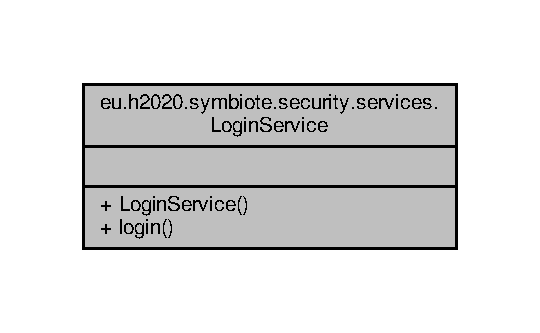
\includegraphics[width=259pt]{classeu_1_1h2020_1_1symbiote_1_1security_1_1services_1_1LoginService__coll__graph}
\end{center}
\end{figure}
\subsection*{Public Member Functions}
\begin{DoxyCompactItemize}
\item 
{\bfseries Login\+Service} (\hyperlink{interfaceeu_1_1h2020_1_1symbiote_1_1security_1_1repositories_1_1UserRepository}{User\+Repository} user\+Repository, \hyperlink{classeu_1_1h2020_1_1symbiote_1_1security_1_1services_1_1TokenService}{Token\+Service} token\+Service, Password\+Encoder password\+Encoder)\hypertarget{classeu_1_1h2020_1_1symbiote_1_1security_1_1services_1_1LoginService_ab115ee7595a83cd9e6c6455c5fe8ef8a}{}\label{classeu_1_1h2020_1_1symbiote_1_1security_1_1services_1_1LoginService_ab115ee7595a83cd9e6c6455c5fe8ef8a}

\item 
Token {\bfseries login} (Credentials user)  throws Missing\+Arguments\+Exception, Wrong\+Credentials\+Exception,             J\+W\+T\+Creation\+Exception \hypertarget{classeu_1_1h2020_1_1symbiote_1_1security_1_1services_1_1LoginService_a6a9c0152923a2526cfb9ecb7b143ad5d}{}\label{classeu_1_1h2020_1_1symbiote_1_1security_1_1services_1_1LoginService_a6a9c0152923a2526cfb9ecb7b143ad5d}

\end{DoxyCompactItemize}


\subsection{Detailed Description}
Spring service used to provide login related functionality of Cloud\+A\+AM.

\begin{DoxyAuthor}{Author}
Daniele Caldarola (C\+N\+IT) 

Nemanja Ignjatov (U\+N\+I\+V\+IE) 

Mikołaj Dobski (P\+S\+NC) 
\end{DoxyAuthor}


The documentation for this class was generated from the following file\+:\begin{DoxyCompactItemize}
\item 
src/main/java/eu/h2020/symbiote/security/services/Login\+Service.\+java\end{DoxyCompactItemize}

\hypertarget{classeu_1_1h2020_1_1symbiote_1_1security_1_1rest_1_1OtherController}{}\section{eu.\+h2020.\+symbiote.\+security.\+rest.\+Other\+Controller Class Reference}
\label{classeu_1_1h2020_1_1symbiote_1_1security_1_1rest_1_1OtherController}\index{eu.\+h2020.\+symbiote.\+security.\+rest.\+Other\+Controller@{eu.\+h2020.\+symbiote.\+security.\+rest.\+Other\+Controller}}


Collaboration diagram for eu.\+h2020.\+symbiote.\+security.\+rest.\+Other\+Controller\+:
\nopagebreak
\begin{figure}[H]
\begin{center}
\leavevmode
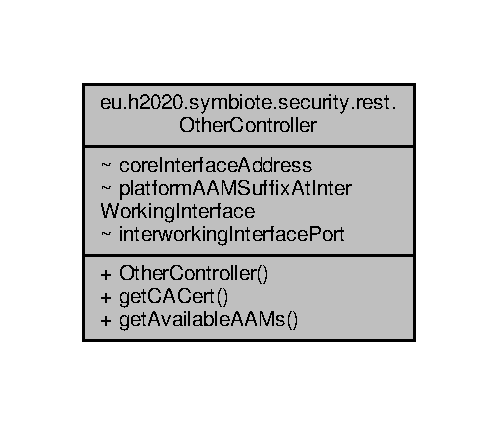
\includegraphics[width=239pt]{classeu_1_1h2020_1_1symbiote_1_1security_1_1rest_1_1OtherController__coll__graph}
\end{center}
\end{figure}
\subsection*{Public Member Functions}
\begin{DoxyCompactItemize}
\item 
{\bfseries Other\+Controller} (\hyperlink{classeu_1_1h2020_1_1symbiote_1_1security_1_1commons_1_1RegistrationManager}{Registration\+Manager} registration\+Manager, \hyperlink{interfaceeu_1_1h2020_1_1symbiote_1_1security_1_1repositories_1_1PlatformRepository}{Platform\+Repository} platform\+Repository)\hypertarget{classeu_1_1h2020_1_1symbiote_1_1security_1_1rest_1_1OtherController_a0de56d515b98dd523cdc6a06b81f8e55}{}\label{classeu_1_1h2020_1_1symbiote_1_1security_1_1rest_1_1OtherController_a0de56d515b98dd523cdc6a06b81f8e55}

\item 
Response\+Entity$<$ String $>$ {\bfseries get\+C\+A\+Cert} ()\hypertarget{classeu_1_1h2020_1_1symbiote_1_1security_1_1rest_1_1OtherController_a124bf65edc033dfebfc58aa757ca2006}{}\label{classeu_1_1h2020_1_1symbiote_1_1security_1_1rest_1_1OtherController_a124bf65edc033dfebfc58aa757ca2006}

\item 
Response\+Entity$<$ List$<$ A\+AM $>$ $>$ {\bfseries get\+Available\+A\+A\+Ms} ()\hypertarget{classeu_1_1h2020_1_1symbiote_1_1security_1_1rest_1_1OtherController_a9b4861233b76f586ad3c45dd92c045ba}{}\label{classeu_1_1h2020_1_1symbiote_1_1security_1_1rest_1_1OtherController_a9b4861233b76f586ad3c45dd92c045ba}

\end{DoxyCompactItemize}


\subsection{Detailed Description}
Spring controller to handle H\+T\+T\+PS requests related to the R\+E\+S\+Tful web service associated to other A\+AM features

\begin{DoxyAuthor}{Author}
Mikołaj Dobski (P\+S\+NC) 
\end{DoxyAuthor}


The documentation for this class was generated from the following file\+:\begin{DoxyCompactItemize}
\item 
src/main/java/eu/h2020/symbiote/security/rest/Other\+Controller.\+java\end{DoxyCompactItemize}

\hypertarget{classeu_1_1h2020_1_1symbiote_1_1security_1_1amqp_1_1consumers_1_1OwnedPlatformDetailsRequestConsumerService}{}\section{eu.\+h2020.\+symbiote.\+security.\+amqp.\+consumers.\+Owned\+Platform\+Details\+Request\+Consumer\+Service Class Reference}
\label{classeu_1_1h2020_1_1symbiote_1_1security_1_1amqp_1_1consumers_1_1OwnedPlatformDetailsRequestConsumerService}\index{eu.\+h2020.\+symbiote.\+security.\+amqp.\+consumers.\+Owned\+Platform\+Details\+Request\+Consumer\+Service@{eu.\+h2020.\+symbiote.\+security.\+amqp.\+consumers.\+Owned\+Platform\+Details\+Request\+Consumer\+Service}}


Inheritance diagram for eu.\+h2020.\+symbiote.\+security.\+amqp.\+consumers.\+Owned\+Platform\+Details\+Request\+Consumer\+Service\+:
\nopagebreak
\begin{figure}[H]
\begin{center}
\leavevmode
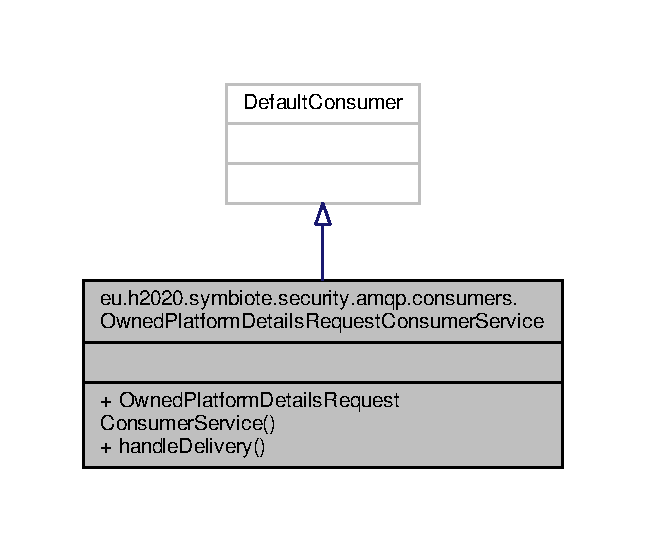
\includegraphics[width=310pt]{classeu_1_1h2020_1_1symbiote_1_1security_1_1amqp_1_1consumers_1_1OwnedPlatformDetailsRequestConsumerService__inherit__graph}
\end{center}
\end{figure}


Collaboration diagram for eu.\+h2020.\+symbiote.\+security.\+amqp.\+consumers.\+Owned\+Platform\+Details\+Request\+Consumer\+Service\+:
\nopagebreak
\begin{figure}[H]
\begin{center}
\leavevmode
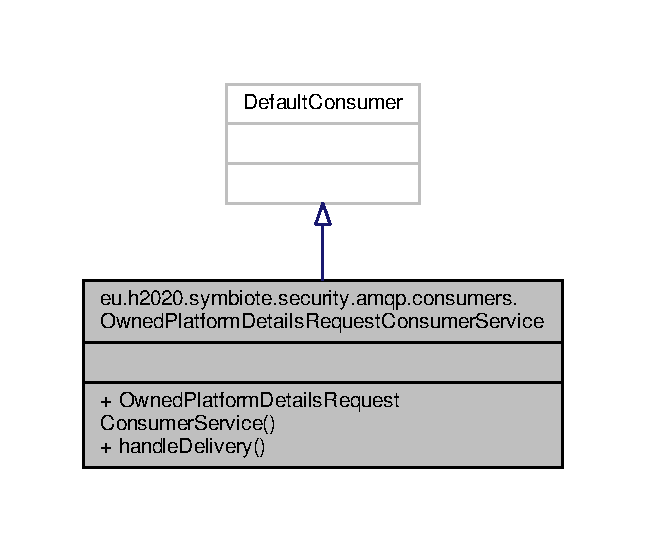
\includegraphics[width=310pt]{classeu_1_1h2020_1_1symbiote_1_1security_1_1amqp_1_1consumers_1_1OwnedPlatformDetailsRequestConsumerService__coll__graph}
\end{center}
\end{figure}
\subsection*{Public Member Functions}
\begin{DoxyCompactItemize}
\item 
\hyperlink{classeu_1_1h2020_1_1symbiote_1_1security_1_1amqp_1_1consumers_1_1OwnedPlatformDetailsRequestConsumerService_a79b32cc135bcb5cdef4783308bdbeffa}{Owned\+Platform\+Details\+Request\+Consumer\+Service} (Channel channel, \hyperlink{interfaceeu_1_1h2020_1_1symbiote_1_1security_1_1repositories_1_1UserRepository}{User\+Repository} user\+Repository, \hyperlink{interfaceeu_1_1h2020_1_1symbiote_1_1security_1_1repositories_1_1PlatformRepository}{Platform\+Repository} platform\+Repository)
\item 
void \hyperlink{classeu_1_1h2020_1_1symbiote_1_1security_1_1amqp_1_1consumers_1_1OwnedPlatformDetailsRequestConsumerService_a910d4de7fd8d139915bd0769ef19262e}{handle\+Delivery} (String consumer\+Tag, Envelope envelope, A\+M\+Q\+P.\+Basic\+Properties properties, byte\mbox{[}$\,$\mbox{]} body)  throws I\+O\+Exception 
\end{DoxyCompactItemize}


\subsection{Detailed Description}
Rabbit\+MQ Consumer implementation used for providing owned platform instances details for the platform owners through Administration module 

\subsection{Constructor \& Destructor Documentation}
\index{eu\+::h2020\+::symbiote\+::security\+::amqp\+::consumers\+::\+Owned\+Platform\+Details\+Request\+Consumer\+Service@{eu\+::h2020\+::symbiote\+::security\+::amqp\+::consumers\+::\+Owned\+Platform\+Details\+Request\+Consumer\+Service}!Owned\+Platform\+Details\+Request\+Consumer\+Service@{Owned\+Platform\+Details\+Request\+Consumer\+Service}}
\index{Owned\+Platform\+Details\+Request\+Consumer\+Service@{Owned\+Platform\+Details\+Request\+Consumer\+Service}!eu\+::h2020\+::symbiote\+::security\+::amqp\+::consumers\+::\+Owned\+Platform\+Details\+Request\+Consumer\+Service@{eu\+::h2020\+::symbiote\+::security\+::amqp\+::consumers\+::\+Owned\+Platform\+Details\+Request\+Consumer\+Service}}
\subsubsection[{\texorpdfstring{Owned\+Platform\+Details\+Request\+Consumer\+Service(\+Channel channel, User\+Repository user\+Repository, Platform\+Repository platform\+Repository)}{OwnedPlatformDetailsRequestConsumerService(Channel channel, UserRepository userRepository, PlatformRepository platformRepository)}}]{\setlength{\rightskip}{0pt plus 5cm}eu.\+h2020.\+symbiote.\+security.\+amqp.\+consumers.\+Owned\+Platform\+Details\+Request\+Consumer\+Service.\+Owned\+Platform\+Details\+Request\+Consumer\+Service (
\begin{DoxyParamCaption}
\item[{Channel}]{channel, }
\item[{{\bf User\+Repository}}]{user\+Repository, }
\item[{{\bf Platform\+Repository}}]{platform\+Repository}
\end{DoxyParamCaption}
)}\hypertarget{classeu_1_1h2020_1_1symbiote_1_1security_1_1amqp_1_1consumers_1_1OwnedPlatformDetailsRequestConsumerService_a79b32cc135bcb5cdef4783308bdbeffa}{}\label{classeu_1_1h2020_1_1symbiote_1_1security_1_1amqp_1_1consumers_1_1OwnedPlatformDetailsRequestConsumerService_a79b32cc135bcb5cdef4783308bdbeffa}
Constructs a new instance and records its association to the passed-\/in channel. Managers beans passed as parameters because of lack of possibility to inject it to consumer.


\begin{DoxyParams}{Parameters}
{\em channel} & the channel to which this consumer is attached \\
\hline
{\em user\+Repository} & \\
\hline
{\em platform\+Repository} & \\
\hline
\end{DoxyParams}


\subsection{Member Function Documentation}
\index{eu\+::h2020\+::symbiote\+::security\+::amqp\+::consumers\+::\+Owned\+Platform\+Details\+Request\+Consumer\+Service@{eu\+::h2020\+::symbiote\+::security\+::amqp\+::consumers\+::\+Owned\+Platform\+Details\+Request\+Consumer\+Service}!handle\+Delivery@{handle\+Delivery}}
\index{handle\+Delivery@{handle\+Delivery}!eu\+::h2020\+::symbiote\+::security\+::amqp\+::consumers\+::\+Owned\+Platform\+Details\+Request\+Consumer\+Service@{eu\+::h2020\+::symbiote\+::security\+::amqp\+::consumers\+::\+Owned\+Platform\+Details\+Request\+Consumer\+Service}}
\subsubsection[{\texorpdfstring{handle\+Delivery(\+String consumer\+Tag, Envelope envelope, A\+M\+Q\+P.\+Basic\+Properties properties, byte[] body)}{handleDelivery(String consumerTag, Envelope envelope, AMQP.BasicProperties properties, byte[] body)}}]{\setlength{\rightskip}{0pt plus 5cm}void eu.\+h2020.\+symbiote.\+security.\+amqp.\+consumers.\+Owned\+Platform\+Details\+Request\+Consumer\+Service.\+handle\+Delivery (
\begin{DoxyParamCaption}
\item[{String}]{consumer\+Tag, }
\item[{Envelope}]{envelope, }
\item[{A\+M\+Q\+P.\+Basic\+Properties}]{properties, }
\item[{byte\mbox{[}$\,$\mbox{]}}]{body}
\end{DoxyParamCaption}
) throws I\+O\+Exception}\hypertarget{classeu_1_1h2020_1_1symbiote_1_1security_1_1amqp_1_1consumers_1_1OwnedPlatformDetailsRequestConsumerService_a910d4de7fd8d139915bd0769ef19262e}{}\label{classeu_1_1h2020_1_1symbiote_1_1security_1_1amqp_1_1consumers_1_1OwnedPlatformDetailsRequestConsumerService_a910d4de7fd8d139915bd0769ef19262e}
Called when a {\ttfamily {\bfseries basic.\+deliver}} is received for this consumer.


\begin{DoxyParams}{Parameters}
{\em consumer\+Tag} & the {\itshape consumer tag} associated with the consumer \\
\hline
{\em envelope} & packaging data for the message \\
\hline
{\em properties} & content header data for the message \\
\hline
{\em body} & the message body (opaque, client-\/specific byte array) \\
\hline
\end{DoxyParams}

\begin{DoxyExceptions}{Exceptions}
{\em I\+O\+Exception} & if the consumer encounters an I/O error while processing the message \\
\hline
\end{DoxyExceptions}
\begin{DoxySeeAlso}{See also}
Envelope 
\end{DoxySeeAlso}


The documentation for this class was generated from the following file\+:\begin{DoxyCompactItemize}
\item 
src/main/java/eu/h2020/symbiote/security/amqp/consumers/Owned\+Platform\+Details\+Request\+Consumer\+Service.\+java\end{DoxyCompactItemize}

\hypertarget{classeu_1_1h2020_1_1symbiote_1_1security_1_1commons_1_1Platform}{}\section{eu.\+h2020.\+symbiote.\+security.\+commons.\+Platform Class Reference}
\label{classeu_1_1h2020_1_1symbiote_1_1security_1_1commons_1_1Platform}\index{eu.\+h2020.\+symbiote.\+security.\+commons.\+Platform@{eu.\+h2020.\+symbiote.\+security.\+commons.\+Platform}}


Collaboration diagram for eu.\+h2020.\+symbiote.\+security.\+commons.\+Platform\+:
\nopagebreak
\begin{figure}[H]
\begin{center}
\leavevmode
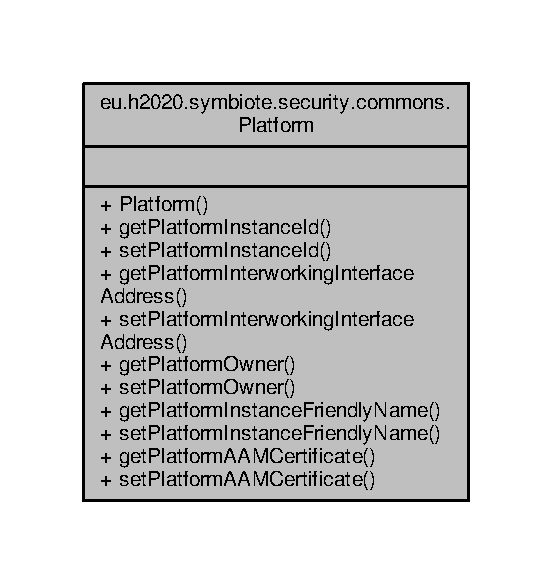
\includegraphics[width=265pt]{classeu_1_1h2020_1_1symbiote_1_1security_1_1commons_1_1Platform__coll__graph}
\end{center}
\end{figure}
\subsection*{Public Member Functions}
\begin{DoxyCompactItemize}
\item 
\hyperlink{classeu_1_1h2020_1_1symbiote_1_1security_1_1commons_1_1Platform_aa19175370c312a3e4409dee595e6b71e}{Platform} (String platform\+Instance\+Id, String platform\+Interworking\+Interface\+Address, String platform\+Instance\+Friendly\+Name, \hyperlink{classeu_1_1h2020_1_1symbiote_1_1security_1_1commons_1_1User}{User} platform\+Owner, Certificate platform\+A\+A\+M\+Certificate)
\item 
String \hyperlink{classeu_1_1h2020_1_1symbiote_1_1security_1_1commons_1_1Platform_ad7ca1891c4c5dc3b52d7fae5138d4e5f}{get\+Platform\+Instance\+Id} ()
\item 
void {\bfseries set\+Platform\+Instance\+Id} (String platform\+Instance\+Id)\hypertarget{classeu_1_1h2020_1_1symbiote_1_1security_1_1commons_1_1Platform_af988ed82685b25a179f7bc7a752041ec}{}\label{classeu_1_1h2020_1_1symbiote_1_1security_1_1commons_1_1Platform_af988ed82685b25a179f7bc7a752041ec}

\item 
String \hyperlink{classeu_1_1h2020_1_1symbiote_1_1security_1_1commons_1_1Platform_acc15f90ae459455e3af02f99fbde1ea0}{get\+Platform\+Interworking\+Interface\+Address} ()
\item 
void {\bfseries set\+Platform\+Interworking\+Interface\+Address} (String platform\+Interworking\+Interface\+Address)\hypertarget{classeu_1_1h2020_1_1symbiote_1_1security_1_1commons_1_1Platform_a623e866018fcb9145cf0405de8811ac4}{}\label{classeu_1_1h2020_1_1symbiote_1_1security_1_1commons_1_1Platform_a623e866018fcb9145cf0405de8811ac4}

\item 
\hyperlink{classeu_1_1h2020_1_1symbiote_1_1security_1_1commons_1_1User}{User} {\bfseries get\+Platform\+Owner} ()\hypertarget{classeu_1_1h2020_1_1symbiote_1_1security_1_1commons_1_1Platform_a91649331565298d271f39a214c802198}{}\label{classeu_1_1h2020_1_1symbiote_1_1security_1_1commons_1_1Platform_a91649331565298d271f39a214c802198}

\item 
void {\bfseries set\+Platform\+Owner} (\hyperlink{classeu_1_1h2020_1_1symbiote_1_1security_1_1commons_1_1User}{User} platform\+Owner)\hypertarget{classeu_1_1h2020_1_1symbiote_1_1security_1_1commons_1_1Platform_a6b186d1add3bd4ea1685b7b004e01ee6}{}\label{classeu_1_1h2020_1_1symbiote_1_1security_1_1commons_1_1Platform_a6b186d1add3bd4ea1685b7b004e01ee6}

\item 
String \hyperlink{classeu_1_1h2020_1_1symbiote_1_1security_1_1commons_1_1Platform_affb694b25f23a3e51ed954ef1cbee285}{get\+Platform\+Instance\+Friendly\+Name} ()
\item 
void {\bfseries set\+Platform\+Instance\+Friendly\+Name} (String platform\+Instance\+Friendly\+Name)\hypertarget{classeu_1_1h2020_1_1symbiote_1_1security_1_1commons_1_1Platform_aa638ef51e567eb7eef993f06202a703a}{}\label{classeu_1_1h2020_1_1symbiote_1_1security_1_1commons_1_1Platform_aa638ef51e567eb7eef993f06202a703a}

\item 
Certificate {\bfseries get\+Platform\+A\+A\+M\+Certificate} ()\hypertarget{classeu_1_1h2020_1_1symbiote_1_1security_1_1commons_1_1Platform_aa6fc0d1badb106432e26ea90f94ee9b5}{}\label{classeu_1_1h2020_1_1symbiote_1_1security_1_1commons_1_1Platform_aa6fc0d1badb106432e26ea90f94ee9b5}

\item 
void {\bfseries set\+Platform\+A\+A\+M\+Certificate} (Certificate platform\+A\+A\+M\+Certificate)\hypertarget{classeu_1_1h2020_1_1symbiote_1_1security_1_1commons_1_1Platform_addc0ccf19ee9e9ffd009184981aca2c6}{}\label{classeu_1_1h2020_1_1symbiote_1_1security_1_1commons_1_1Platform_addc0ccf19ee9e9ffd009184981aca2c6}

\end{DoxyCompactItemize}


\subsection{Detailed Description}
Symb\+Io\+Te-\/enabled IoT platform instance registered in the Core A\+AM.

\begin{DoxyAuthor}{Author}
Mikołaj Dobski (P\+S\+NC) 
\end{DoxyAuthor}


\subsection{Constructor \& Destructor Documentation}
\index{eu\+::h2020\+::symbiote\+::security\+::commons\+::\+Platform@{eu\+::h2020\+::symbiote\+::security\+::commons\+::\+Platform}!Platform@{Platform}}
\index{Platform@{Platform}!eu\+::h2020\+::symbiote\+::security\+::commons\+::\+Platform@{eu\+::h2020\+::symbiote\+::security\+::commons\+::\+Platform}}
\subsubsection[{\texorpdfstring{Platform(\+String platform\+Instance\+Id, String platform\+Interworking\+Interface\+Address, String platform\+Instance\+Friendly\+Name, User platform\+Owner, Certificate platform\+A\+A\+M\+Certificate)}{Platform(String platformInstanceId, String platformInterworkingInterfaceAddress, String platformInstanceFriendlyName, User platformOwner, Certificate platformAAMCertificate)}}]{\setlength{\rightskip}{0pt plus 5cm}eu.\+h2020.\+symbiote.\+security.\+commons.\+Platform.\+Platform (
\begin{DoxyParamCaption}
\item[{String}]{platform\+Instance\+Id, }
\item[{String}]{platform\+Interworking\+Interface\+Address, }
\item[{String}]{platform\+Instance\+Friendly\+Name, }
\item[{{\bf User}}]{platform\+Owner, }
\item[{Certificate}]{platform\+A\+A\+M\+Certificate}
\end{DoxyParamCaption}
)}\hypertarget{classeu_1_1h2020_1_1symbiote_1_1security_1_1commons_1_1Platform_aa19175370c312a3e4409dee595e6b71e}{}\label{classeu_1_1h2020_1_1symbiote_1_1security_1_1commons_1_1Platform_aa19175370c312a3e4409dee595e6b71e}

\begin{DoxyParams}{Parameters}
{\em platform\+Instance\+Id} & Symb\+Io\+Te-\/unique platform identifier \\
\hline
{\em platform\+Interworking\+Interface\+Address} & Address where the \hyperlink{classeu_1_1h2020_1_1symbiote_1_1security_1_1commons_1_1Platform}{Platform} exposes its Interworking Interface \\
\hline
{\em platform\+Instance\+Friendly\+Name} & a label for the end user to be able to identify the login endrypoint \\
\hline
{\em platform\+Owner} & details of the \hyperlink{classeu_1_1h2020_1_1symbiote_1_1security_1_1commons_1_1Platform}{Platform} Owner \\
\hline
\end{DoxyParams}


\subsection{Member Function Documentation}
\index{eu\+::h2020\+::symbiote\+::security\+::commons\+::\+Platform@{eu\+::h2020\+::symbiote\+::security\+::commons\+::\+Platform}!get\+Platform\+Instance\+Friendly\+Name@{get\+Platform\+Instance\+Friendly\+Name}}
\index{get\+Platform\+Instance\+Friendly\+Name@{get\+Platform\+Instance\+Friendly\+Name}!eu\+::h2020\+::symbiote\+::security\+::commons\+::\+Platform@{eu\+::h2020\+::symbiote\+::security\+::commons\+::\+Platform}}
\subsubsection[{\texorpdfstring{get\+Platform\+Instance\+Friendly\+Name()}{getPlatformInstanceFriendlyName()}}]{\setlength{\rightskip}{0pt plus 5cm}String eu.\+h2020.\+symbiote.\+security.\+commons.\+Platform.\+get\+Platform\+Instance\+Friendly\+Name (
\begin{DoxyParamCaption}
{}
\end{DoxyParamCaption}
)}\hypertarget{classeu_1_1h2020_1_1symbiote_1_1security_1_1commons_1_1Platform_affb694b25f23a3e51ed954ef1cbee285}{}\label{classeu_1_1h2020_1_1symbiote_1_1security_1_1commons_1_1Platform_affb694b25f23a3e51ed954ef1cbee285}
\begin{DoxyReturn}{Returns}
a label for the end user to be able to identify the login endrypoint 
\end{DoxyReturn}
\index{eu\+::h2020\+::symbiote\+::security\+::commons\+::\+Platform@{eu\+::h2020\+::symbiote\+::security\+::commons\+::\+Platform}!get\+Platform\+Instance\+Id@{get\+Platform\+Instance\+Id}}
\index{get\+Platform\+Instance\+Id@{get\+Platform\+Instance\+Id}!eu\+::h2020\+::symbiote\+::security\+::commons\+::\+Platform@{eu\+::h2020\+::symbiote\+::security\+::commons\+::\+Platform}}
\subsubsection[{\texorpdfstring{get\+Platform\+Instance\+Id()}{getPlatformInstanceId()}}]{\setlength{\rightskip}{0pt plus 5cm}String eu.\+h2020.\+symbiote.\+security.\+commons.\+Platform.\+get\+Platform\+Instance\+Id (
\begin{DoxyParamCaption}
{}
\end{DoxyParamCaption}
)}\hypertarget{classeu_1_1h2020_1_1symbiote_1_1security_1_1commons_1_1Platform_ad7ca1891c4c5dc3b52d7fae5138d4e5f}{}\label{classeu_1_1h2020_1_1symbiote_1_1security_1_1commons_1_1Platform_ad7ca1891c4c5dc3b52d7fae5138d4e5f}
\begin{DoxyReturn}{Returns}
Symb\+Io\+Te-\/unique platform identifier 
\end{DoxyReturn}
\index{eu\+::h2020\+::symbiote\+::security\+::commons\+::\+Platform@{eu\+::h2020\+::symbiote\+::security\+::commons\+::\+Platform}!get\+Platform\+Interworking\+Interface\+Address@{get\+Platform\+Interworking\+Interface\+Address}}
\index{get\+Platform\+Interworking\+Interface\+Address@{get\+Platform\+Interworking\+Interface\+Address}!eu\+::h2020\+::symbiote\+::security\+::commons\+::\+Platform@{eu\+::h2020\+::symbiote\+::security\+::commons\+::\+Platform}}
\subsubsection[{\texorpdfstring{get\+Platform\+Interworking\+Interface\+Address()}{getPlatformInterworkingInterfaceAddress()}}]{\setlength{\rightskip}{0pt plus 5cm}String eu.\+h2020.\+symbiote.\+security.\+commons.\+Platform.\+get\+Platform\+Interworking\+Interface\+Address (
\begin{DoxyParamCaption}
{}
\end{DoxyParamCaption}
)}\hypertarget{classeu_1_1h2020_1_1symbiote_1_1security_1_1commons_1_1Platform_acc15f90ae459455e3af02f99fbde1ea0}{}\label{classeu_1_1h2020_1_1symbiote_1_1security_1_1commons_1_1Platform_acc15f90ae459455e3af02f99fbde1ea0}
\begin{DoxyReturn}{Returns}
Address where the \hyperlink{classeu_1_1h2020_1_1symbiote_1_1security_1_1commons_1_1Platform}{Platform} exposes its Interworking Interface 
\end{DoxyReturn}


The documentation for this class was generated from the following file\+:\begin{DoxyCompactItemize}
\item 
src/main/java/eu/h2020/symbiote/security/commons/Platform.\+java\end{DoxyCompactItemize}

\hypertarget{classeu_1_1h2020_1_1symbiote_1_1security_1_1amqp_1_1consumers_1_1PlatformRegistrationRequestConsumerService}{}\section{eu.\+h2020.\+symbiote.\+security.\+amqp.\+consumers.\+Platform\+Registration\+Request\+Consumer\+Service Class Reference}
\label{classeu_1_1h2020_1_1symbiote_1_1security_1_1amqp_1_1consumers_1_1PlatformRegistrationRequestConsumerService}\index{eu.\+h2020.\+symbiote.\+security.\+amqp.\+consumers.\+Platform\+Registration\+Request\+Consumer\+Service@{eu.\+h2020.\+symbiote.\+security.\+amqp.\+consumers.\+Platform\+Registration\+Request\+Consumer\+Service}}


Inheritance diagram for eu.\+h2020.\+symbiote.\+security.\+amqp.\+consumers.\+Platform\+Registration\+Request\+Consumer\+Service\+:
\nopagebreak
\begin{figure}[H]
\begin{center}
\leavevmode
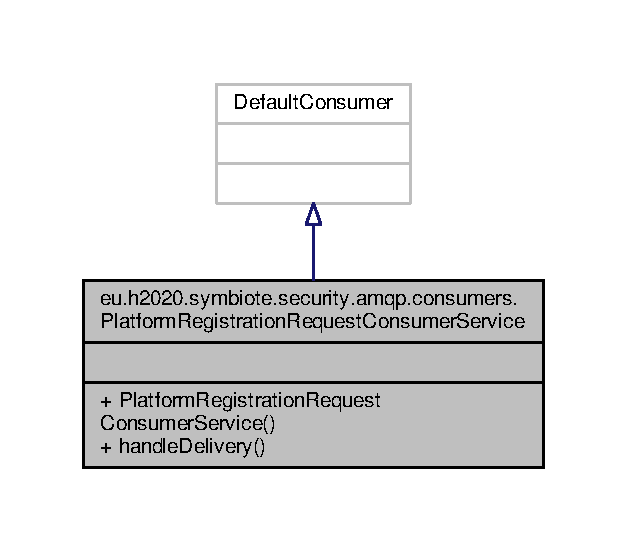
\includegraphics[width=301pt]{classeu_1_1h2020_1_1symbiote_1_1security_1_1amqp_1_1consumers_1_1PlatformRegistrationRequestConsumerService__inherit__graph}
\end{center}
\end{figure}


Collaboration diagram for eu.\+h2020.\+symbiote.\+security.\+amqp.\+consumers.\+Platform\+Registration\+Request\+Consumer\+Service\+:
\nopagebreak
\begin{figure}[H]
\begin{center}
\leavevmode
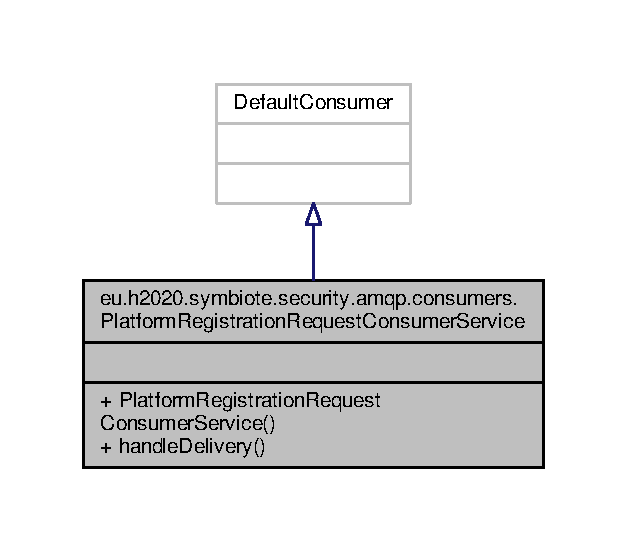
\includegraphics[width=301pt]{classeu_1_1h2020_1_1symbiote_1_1security_1_1amqp_1_1consumers_1_1PlatformRegistrationRequestConsumerService__coll__graph}
\end{center}
\end{figure}
\subsection*{Public Member Functions}
\begin{DoxyCompactItemize}
\item 
\hyperlink{classeu_1_1h2020_1_1symbiote_1_1security_1_1amqp_1_1consumers_1_1PlatformRegistrationRequestConsumerService_ade7d1c51240268d9f63a02d5cb4faf5c}{Platform\+Registration\+Request\+Consumer\+Service} (Channel channel, \hyperlink{classeu_1_1h2020_1_1symbiote_1_1security_1_1services_1_1PlatformRegistrationService}{Platform\+Registration\+Service} platform\+Registration\+Service)
\item 
void \hyperlink{classeu_1_1h2020_1_1symbiote_1_1security_1_1amqp_1_1consumers_1_1PlatformRegistrationRequestConsumerService_a69334c874254fa8b50a3f7db6665aed8}{handle\+Delivery} (String consumer\+Tag, Envelope envelope, A\+M\+Q\+P.\+Basic\+Properties properties, byte\mbox{[}$\,$\mbox{]} body)  throws I\+O\+Exception 
\end{DoxyCompactItemize}


\subsection{Detailed Description}
Rabbit\+MQ Consumer implementation used for Platforms\textquotesingle{} Registration actions

\begin{DoxyAuthor}{Author}
Mikołaj Dobski (P\+S\+NC) 
\end{DoxyAuthor}


\subsection{Constructor \& Destructor Documentation}
\index{eu\+::h2020\+::symbiote\+::security\+::amqp\+::consumers\+::\+Platform\+Registration\+Request\+Consumer\+Service@{eu\+::h2020\+::symbiote\+::security\+::amqp\+::consumers\+::\+Platform\+Registration\+Request\+Consumer\+Service}!Platform\+Registration\+Request\+Consumer\+Service@{Platform\+Registration\+Request\+Consumer\+Service}}
\index{Platform\+Registration\+Request\+Consumer\+Service@{Platform\+Registration\+Request\+Consumer\+Service}!eu\+::h2020\+::symbiote\+::security\+::amqp\+::consumers\+::\+Platform\+Registration\+Request\+Consumer\+Service@{eu\+::h2020\+::symbiote\+::security\+::amqp\+::consumers\+::\+Platform\+Registration\+Request\+Consumer\+Service}}
\subsubsection[{\texorpdfstring{Platform\+Registration\+Request\+Consumer\+Service(\+Channel channel, Platform\+Registration\+Service platform\+Registration\+Service)}{PlatformRegistrationRequestConsumerService(Channel channel, PlatformRegistrationService platformRegistrationService)}}]{\setlength{\rightskip}{0pt plus 5cm}eu.\+h2020.\+symbiote.\+security.\+amqp.\+consumers.\+Platform\+Registration\+Request\+Consumer\+Service.\+Platform\+Registration\+Request\+Consumer\+Service (
\begin{DoxyParamCaption}
\item[{Channel}]{channel, }
\item[{{\bf Platform\+Registration\+Service}}]{platform\+Registration\+Service}
\end{DoxyParamCaption}
)}\hypertarget{classeu_1_1h2020_1_1symbiote_1_1security_1_1amqp_1_1consumers_1_1PlatformRegistrationRequestConsumerService_ade7d1c51240268d9f63a02d5cb4faf5c}{}\label{classeu_1_1h2020_1_1symbiote_1_1security_1_1amqp_1_1consumers_1_1PlatformRegistrationRequestConsumerService_ade7d1c51240268d9f63a02d5cb4faf5c}
Constructs a new instance and records its association to the passed-\/in channel. Managers beans passed as parameters because of lack of possibility to inject it to consumer.


\begin{DoxyParams}{Parameters}
{\em channel} & the channel to which this consumer is attached \\
\hline
\end{DoxyParams}


\subsection{Member Function Documentation}
\index{eu\+::h2020\+::symbiote\+::security\+::amqp\+::consumers\+::\+Platform\+Registration\+Request\+Consumer\+Service@{eu\+::h2020\+::symbiote\+::security\+::amqp\+::consumers\+::\+Platform\+Registration\+Request\+Consumer\+Service}!handle\+Delivery@{handle\+Delivery}}
\index{handle\+Delivery@{handle\+Delivery}!eu\+::h2020\+::symbiote\+::security\+::amqp\+::consumers\+::\+Platform\+Registration\+Request\+Consumer\+Service@{eu\+::h2020\+::symbiote\+::security\+::amqp\+::consumers\+::\+Platform\+Registration\+Request\+Consumer\+Service}}
\subsubsection[{\texorpdfstring{handle\+Delivery(\+String consumer\+Tag, Envelope envelope, A\+M\+Q\+P.\+Basic\+Properties properties, byte[] body)}{handleDelivery(String consumerTag, Envelope envelope, AMQP.BasicProperties properties, byte[] body)}}]{\setlength{\rightskip}{0pt plus 5cm}void eu.\+h2020.\+symbiote.\+security.\+amqp.\+consumers.\+Platform\+Registration\+Request\+Consumer\+Service.\+handle\+Delivery (
\begin{DoxyParamCaption}
\item[{String}]{consumer\+Tag, }
\item[{Envelope}]{envelope, }
\item[{A\+M\+Q\+P.\+Basic\+Properties}]{properties, }
\item[{byte\mbox{[}$\,$\mbox{]}}]{body}
\end{DoxyParamCaption}
) throws I\+O\+Exception}\hypertarget{classeu_1_1h2020_1_1symbiote_1_1security_1_1amqp_1_1consumers_1_1PlatformRegistrationRequestConsumerService_a69334c874254fa8b50a3f7db6665aed8}{}\label{classeu_1_1h2020_1_1symbiote_1_1security_1_1amqp_1_1consumers_1_1PlatformRegistrationRequestConsumerService_a69334c874254fa8b50a3f7db6665aed8}
Called when a {\ttfamily {\bfseries basic.\+deliver}} is received for this consumer.


\begin{DoxyParams}{Parameters}
{\em consumer\+Tag} & the {\itshape consumer tag} associated with the consumer \\
\hline
{\em envelope} & packaging data for the message \\
\hline
{\em properties} & content header data for the message \\
\hline
{\em body} & the message body (opaque, client-\/specific byte array) \\
\hline
\end{DoxyParams}

\begin{DoxyExceptions}{Exceptions}
{\em I\+O\+Exception} & if the consumer encounters an I/O error while processing the message \\
\hline
\end{DoxyExceptions}
\begin{DoxySeeAlso}{See also}
Envelope 
\end{DoxySeeAlso}


The documentation for this class was generated from the following file\+:\begin{DoxyCompactItemize}
\item 
src/main/java/eu/h2020/symbiote/security/amqp/consumers/Platform\+Registration\+Request\+Consumer\+Service.\+java\end{DoxyCompactItemize}

\hypertarget{classeu_1_1h2020_1_1symbiote_1_1security_1_1services_1_1PlatformRegistrationService}{}\section{eu.\+h2020.\+symbiote.\+security.\+services.\+Platform\+Registration\+Service Class Reference}
\label{classeu_1_1h2020_1_1symbiote_1_1security_1_1services_1_1PlatformRegistrationService}\index{eu.\+h2020.\+symbiote.\+security.\+services.\+Platform\+Registration\+Service@{eu.\+h2020.\+symbiote.\+security.\+services.\+Platform\+Registration\+Service}}


Collaboration diagram for eu.\+h2020.\+symbiote.\+security.\+services.\+Platform\+Registration\+Service\+:
\nopagebreak
\begin{figure}[H]
\begin{center}
\leavevmode
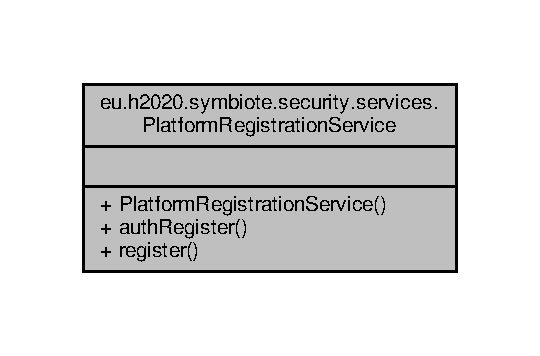
\includegraphics[width=259pt]{classeu_1_1h2020_1_1symbiote_1_1security_1_1services_1_1PlatformRegistrationService__coll__graph}
\end{center}
\end{figure}
\subsection*{Public Member Functions}
\begin{DoxyCompactItemize}
\item 
{\bfseries Platform\+Registration\+Service} (\hyperlink{interfaceeu_1_1h2020_1_1symbiote_1_1security_1_1repositories_1_1UserRepository}{User\+Repository} user\+Repository, \hyperlink{classeu_1_1h2020_1_1symbiote_1_1security_1_1services_1_1UserRegistrationService}{User\+Registration\+Service} user\+Registration\+Service, \hyperlink{interfaceeu_1_1h2020_1_1symbiote_1_1security_1_1repositories_1_1PlatformRepository}{Platform\+Repository} platform\+Repository, \hyperlink{classeu_1_1h2020_1_1symbiote_1_1security_1_1commons_1_1RegistrationManager}{Registration\+Manager} registration\+Manager)\hypertarget{classeu_1_1h2020_1_1symbiote_1_1security_1_1services_1_1PlatformRegistrationService_a3ec750fd2f40e2c9ea5b9090826f49d5}{}\label{classeu_1_1h2020_1_1symbiote_1_1security_1_1services_1_1PlatformRegistrationService_a3ec750fd2f40e2c9ea5b9090826f49d5}

\item 
Platform\+Registration\+Response {\bfseries auth\+Register} (Platform\+Registration\+Request request)  throws A\+A\+M\+Exception \hypertarget{classeu_1_1h2020_1_1symbiote_1_1security_1_1services_1_1PlatformRegistrationService_a1ff8016dbe7d30d98cfd965b7abc044f}{}\label{classeu_1_1h2020_1_1symbiote_1_1security_1_1services_1_1PlatformRegistrationService_a1ff8016dbe7d30d98cfd965b7abc044f}

\item 
Platform\+Registration\+Response {\bfseries register} (Platform\+Registration\+Request platform\+Registration\+Request)  throws A\+A\+M\+Exception \hypertarget{classeu_1_1h2020_1_1symbiote_1_1security_1_1services_1_1PlatformRegistrationService_a07e05bad6ada1c9e1152dd61de6c5f50}{}\label{classeu_1_1h2020_1_1symbiote_1_1security_1_1services_1_1PlatformRegistrationService_a07e05bad6ada1c9e1152dd61de6c5f50}

\end{DoxyCompactItemize}


\subsection{Detailed Description}
Spring service used to register platforms and their owners in the A\+AM repository.

\begin{DoxyAuthor}{Author}
Mikołaj Dobski (P\+S\+NC) 
\end{DoxyAuthor}


The documentation for this class was generated from the following file\+:\begin{DoxyCompactItemize}
\item 
src/main/java/eu/h2020/symbiote/security/services/Platform\+Registration\+Service.\+java\end{DoxyCompactItemize}

\hypertarget{interfaceeu_1_1h2020_1_1symbiote_1_1security_1_1repositories_1_1PlatformRepository}{}\section{eu.\+h2020.\+symbiote.\+security.\+repositories.\+Platform\+Repository Interface Reference}
\label{interfaceeu_1_1h2020_1_1symbiote_1_1security_1_1repositories_1_1PlatformRepository}\index{eu.\+h2020.\+symbiote.\+security.\+repositories.\+Platform\+Repository@{eu.\+h2020.\+symbiote.\+security.\+repositories.\+Platform\+Repository}}


Inheritance diagram for eu.\+h2020.\+symbiote.\+security.\+repositories.\+Platform\+Repository\+:
\nopagebreak
\begin{figure}[H]
\begin{center}
\leavevmode
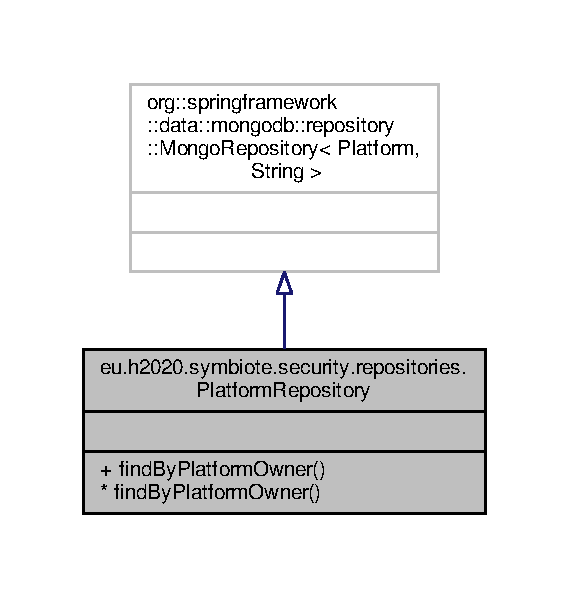
\includegraphics[width=273pt]{interfaceeu_1_1h2020_1_1symbiote_1_1security_1_1repositories_1_1PlatformRepository__inherit__graph}
\end{center}
\end{figure}


Collaboration diagram for eu.\+h2020.\+symbiote.\+security.\+repositories.\+Platform\+Repository\+:
\nopagebreak
\begin{figure}[H]
\begin{center}
\leavevmode
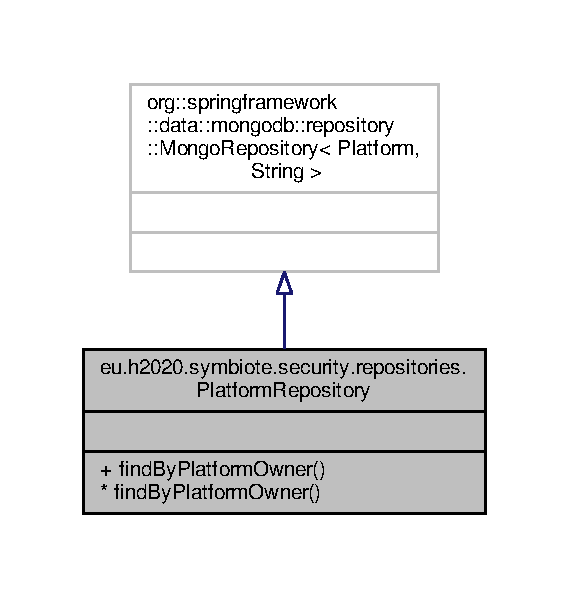
\includegraphics[width=273pt]{interfaceeu_1_1h2020_1_1symbiote_1_1security_1_1repositories_1_1PlatformRepository__coll__graph}
\end{center}
\end{figure}
\subsection*{Public Member Functions}
{\bf }\par
\begin{DoxyCompactItemize}
\item 
\hyperlink{classeu_1_1h2020_1_1symbiote_1_1security_1_1commons_1_1Platform}{Platform} \hyperlink{interfaceeu_1_1h2020_1_1symbiote_1_1security_1_1repositories_1_1PlatformRepository_ae228958e2a7305371e5fca9fd8f9f042}{find\+By\+Platform\+Owner} (\hyperlink{classeu_1_1h2020_1_1symbiote_1_1security_1_1commons_1_1User}{User} platform\+Owner)
\end{DoxyCompactItemize}



\subsection{Detailed Description}
Spring repository interface definition to be used with Mongo\+DB for operations on \hyperlink{}{Platform} entities.

\begin{DoxyAuthor}{Author}
Mikołaj Dobski (P\+S\+NC) 
\end{DoxyAuthor}


\subsection{Member Function Documentation}
\index{eu\+::h2020\+::symbiote\+::security\+::repositories\+::\+Platform\+Repository@{eu\+::h2020\+::symbiote\+::security\+::repositories\+::\+Platform\+Repository}!find\+By\+Platform\+Owner@{find\+By\+Platform\+Owner}}
\index{find\+By\+Platform\+Owner@{find\+By\+Platform\+Owner}!eu\+::h2020\+::symbiote\+::security\+::repositories\+::\+Platform\+Repository@{eu\+::h2020\+::symbiote\+::security\+::repositories\+::\+Platform\+Repository}}
\subsubsection[{\texorpdfstring{find\+By\+Platform\+Owner(\+User platform\+Owner)}{findByPlatformOwner(User platformOwner)}}]{\setlength{\rightskip}{0pt plus 5cm}{\bf Platform} eu.\+h2020.\+symbiote.\+security.\+repositories.\+Platform\+Repository.\+find\+By\+Platform\+Owner (
\begin{DoxyParamCaption}
\item[{{\bf User}}]{platform\+Owner}
\end{DoxyParamCaption}
)}\hypertarget{interfaceeu_1_1h2020_1_1symbiote_1_1security_1_1repositories_1_1PlatformRepository_ae228958e2a7305371e5fca9fd8f9f042}{}\label{interfaceeu_1_1h2020_1_1symbiote_1_1security_1_1repositories_1_1PlatformRepository_ae228958e2a7305371e5fca9fd8f9f042}
Used to retrieve platform from repository knowing its Platform\+Owner\hyperlink{}{\}  platform\+Owner user responsible for this platform   Platform\} related with the given user }

The documentation for this interface was generated from the following file\+:\begin{DoxyCompactItemize}
\item 
src/main/java/eu/h2020/symbiote/security/repositories/Platform\+Repository.\+java\end{DoxyCompactItemize}

\hypertarget{classeu_1_1h2020_1_1symbiote_1_1security_1_1amqp_1_1RabbitManager}{}\section{eu.\+h2020.\+symbiote.\+security.\+amqp.\+Rabbit\+Manager Class Reference}
\label{classeu_1_1h2020_1_1symbiote_1_1security_1_1amqp_1_1RabbitManager}\index{eu.\+h2020.\+symbiote.\+security.\+amqp.\+Rabbit\+Manager@{eu.\+h2020.\+symbiote.\+security.\+amqp.\+Rabbit\+Manager}}


Collaboration diagram for eu.\+h2020.\+symbiote.\+security.\+amqp.\+Rabbit\+Manager\+:
\nopagebreak
\begin{figure}[H]
\begin{center}
\leavevmode
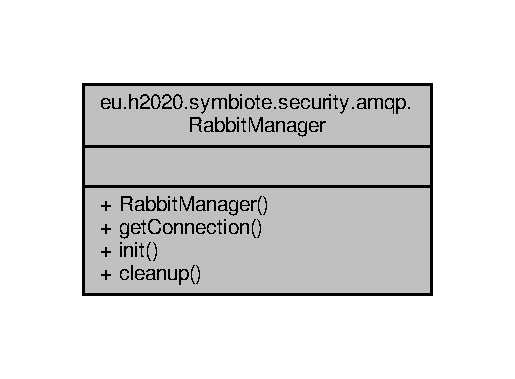
\includegraphics[width=247pt]{classeu_1_1h2020_1_1symbiote_1_1security_1_1amqp_1_1RabbitManager__coll__graph}
\end{center}
\end{figure}
\subsection*{Public Member Functions}
\begin{DoxyCompactItemize}
\item 
{\bfseries Rabbit\+Manager} (\hyperlink{classeu_1_1h2020_1_1symbiote_1_1security_1_1services_1_1UserRegistrationService}{User\+Registration\+Service} user\+Registration\+Service, \hyperlink{classeu_1_1h2020_1_1symbiote_1_1security_1_1services_1_1PlatformRegistrationService}{Platform\+Registration\+Service} platform\+Registration\+Service, \hyperlink{classeu_1_1h2020_1_1symbiote_1_1security_1_1services_1_1LoginService}{Login\+Service} login\+Service, \hyperlink{classeu_1_1h2020_1_1symbiote_1_1security_1_1services_1_1TokenService}{Token\+Service} token\+Service, \hyperlink{interfaceeu_1_1h2020_1_1symbiote_1_1security_1_1repositories_1_1UserRepository}{User\+Repository} user\+Repository, \hyperlink{interfaceeu_1_1h2020_1_1symbiote_1_1security_1_1repositories_1_1PlatformRepository}{Platform\+Repository} platform\+Repository, \hyperlink{classeu_1_1h2020_1_1symbiote_1_1security_1_1commons_1_1RegistrationManager}{Registration\+Manager} registration\+Manager)\hypertarget{classeu_1_1h2020_1_1symbiote_1_1security_1_1amqp_1_1RabbitManager_a20251a4a97883cabfcfbdde90bd293f3}{}\label{classeu_1_1h2020_1_1symbiote_1_1security_1_1amqp_1_1RabbitManager_a20251a4a97883cabfcfbdde90bd293f3}

\item 
Connection \hyperlink{classeu_1_1h2020_1_1symbiote_1_1security_1_1amqp_1_1RabbitManager_a135b27190102885449f08bb49f514a90}{get\+Connection} ()  throws I\+O\+Exception, Timeout\+Exception 
\item 
void \hyperlink{classeu_1_1h2020_1_1symbiote_1_1security_1_1amqp_1_1RabbitManager_a85df036a5614d190f3002b15af43e437}{init} ()  throws A\+A\+M\+Misconfiguration\+Exception 
\item 
void {\bfseries cleanup} ()\hypertarget{classeu_1_1h2020_1_1symbiote_1_1security_1_1amqp_1_1RabbitManager_ab248e0618bcf289a988c130459032b1e}{}\label{classeu_1_1h2020_1_1symbiote_1_1security_1_1amqp_1_1RabbitManager_ab248e0618bcf289a988c130459032b1e}

\end{DoxyCompactItemize}


\subsection{Member Function Documentation}
\index{eu\+::h2020\+::symbiote\+::security\+::amqp\+::\+Rabbit\+Manager@{eu\+::h2020\+::symbiote\+::security\+::amqp\+::\+Rabbit\+Manager}!get\+Connection@{get\+Connection}}
\index{get\+Connection@{get\+Connection}!eu\+::h2020\+::symbiote\+::security\+::amqp\+::\+Rabbit\+Manager@{eu\+::h2020\+::symbiote\+::security\+::amqp\+::\+Rabbit\+Manager}}
\subsubsection[{\texorpdfstring{get\+Connection()}{getConnection()}}]{\setlength{\rightskip}{0pt plus 5cm}Connection eu.\+h2020.\+symbiote.\+security.\+amqp.\+Rabbit\+Manager.\+get\+Connection (
\begin{DoxyParamCaption}
{}
\end{DoxyParamCaption}
) throws I\+O\+Exception, Timeout\+Exception}\hypertarget{classeu_1_1h2020_1_1symbiote_1_1security_1_1amqp_1_1RabbitManager_a135b27190102885449f08bb49f514a90}{}\label{classeu_1_1h2020_1_1symbiote_1_1security_1_1amqp_1_1RabbitManager_a135b27190102885449f08bb49f514a90}
Initiates connection with Rabbit server using parameters from Bootstrap Properties


\begin{DoxyExceptions}{Exceptions}
{\em I\+O\+Exception} & \\
\hline
{\em Timeout\+Exception} & \\
\hline
\end{DoxyExceptions}
\index{eu\+::h2020\+::symbiote\+::security\+::amqp\+::\+Rabbit\+Manager@{eu\+::h2020\+::symbiote\+::security\+::amqp\+::\+Rabbit\+Manager}!init@{init}}
\index{init@{init}!eu\+::h2020\+::symbiote\+::security\+::amqp\+::\+Rabbit\+Manager@{eu\+::h2020\+::symbiote\+::security\+::amqp\+::\+Rabbit\+Manager}}
\subsubsection[{\texorpdfstring{init()}{init()}}]{\setlength{\rightskip}{0pt plus 5cm}void eu.\+h2020.\+symbiote.\+security.\+amqp.\+Rabbit\+Manager.\+init (
\begin{DoxyParamCaption}
{}
\end{DoxyParamCaption}
) throws A\+A\+M\+Misconfiguration\+Exception}\hypertarget{classeu_1_1h2020_1_1symbiote_1_1security_1_1amqp_1_1RabbitManager_a85df036a5614d190f3002b15af43e437}{}\label{classeu_1_1h2020_1_1symbiote_1_1security_1_1amqp_1_1RabbitManager_a85df036a5614d190f3002b15af43e437}
Method creates channel and declares Rabbit exchanges for A\+AM features. It triggers start of all consumers used in with A\+AM communication. 

The documentation for this class was generated from the following file\+:\begin{DoxyCompactItemize}
\item 
src/main/java/eu/h2020/symbiote/security/amqp/Rabbit\+Manager.\+java\end{DoxyCompactItemize}

\hypertarget{classeu_1_1h2020_1_1symbiote_1_1security_1_1commons_1_1RegistrationManager}{}\section{eu.\+h2020.\+symbiote.\+security.\+commons.\+Registration\+Manager Class Reference}
\label{classeu_1_1h2020_1_1symbiote_1_1security_1_1commons_1_1RegistrationManager}\index{eu.\+h2020.\+symbiote.\+security.\+commons.\+Registration\+Manager@{eu.\+h2020.\+symbiote.\+security.\+commons.\+Registration\+Manager}}


Collaboration diagram for eu.\+h2020.\+symbiote.\+security.\+commons.\+Registration\+Manager\+:
\nopagebreak
\begin{figure}[H]
\begin{center}
\leavevmode
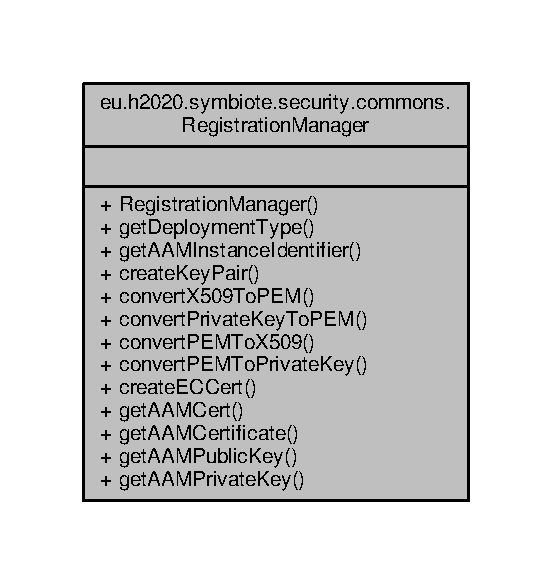
\includegraphics[width=265pt]{classeu_1_1h2020_1_1symbiote_1_1security_1_1commons_1_1RegistrationManager__coll__graph}
\end{center}
\end{figure}
\subsection*{Public Member Functions}
\begin{DoxyCompactItemize}
\item 
Issuing\+Authority\+Type \hyperlink{classeu_1_1h2020_1_1symbiote_1_1security_1_1commons_1_1RegistrationManager_a91aae367f791d2443bc515b2a1e85e6c}{get\+Deployment\+Type} ()
\item 
String \hyperlink{classeu_1_1h2020_1_1symbiote_1_1security_1_1commons_1_1RegistrationManager_a913089ea97d7dc5e4ad18456732cf518}{get\+A\+A\+M\+Instance\+Identifier} ()
\item 
Key\+Pair {\bfseries create\+Key\+Pair} ()  throws No\+Such\+Provider\+Exception, No\+Such\+Algorithm\+Exception,             Invalid\+Algorithm\+Parameter\+Exception \hypertarget{classeu_1_1h2020_1_1symbiote_1_1security_1_1commons_1_1RegistrationManager_ab6d69999be9f251c5e8d8d99539a1d09}{}\label{classeu_1_1h2020_1_1symbiote_1_1security_1_1commons_1_1RegistrationManager_ab6d69999be9f251c5e8d8d99539a1d09}

\item 
String {\bfseries convert\+X509\+To\+P\+EM} (X509\+Certificate signed\+Certificate)  throws I\+O\+Exception \hypertarget{classeu_1_1h2020_1_1symbiote_1_1security_1_1commons_1_1RegistrationManager_a9cc618e3776ae6003c97e4f78359c1f6}{}\label{classeu_1_1h2020_1_1symbiote_1_1security_1_1commons_1_1RegistrationManager_a9cc618e3776ae6003c97e4f78359c1f6}

\item 
String {\bfseries convert\+Private\+Key\+To\+P\+EM} (Private\+Key private\+Key)  throws I\+O\+Exception \hypertarget{classeu_1_1h2020_1_1symbiote_1_1security_1_1commons_1_1RegistrationManager_aa4d9b397346819f854e658f753bb6327}{}\label{classeu_1_1h2020_1_1symbiote_1_1security_1_1commons_1_1RegistrationManager_aa4d9b397346819f854e658f753bb6327}

\item 
X509\+Certificate {\bfseries convert\+P\+E\+M\+To\+X509} (String pem\+Certificate)  throws I\+O\+Exception, Certificate\+Exception \hypertarget{classeu_1_1h2020_1_1symbiote_1_1security_1_1commons_1_1RegistrationManager_a4cd2fc240d24c8d3516960115565d34f}{}\label{classeu_1_1h2020_1_1symbiote_1_1security_1_1commons_1_1RegistrationManager_a4cd2fc240d24c8d3516960115565d34f}

\item 
Private\+Key {\bfseries convert\+P\+E\+M\+To\+Private\+Key} (String pem\+Privatekey)  throws I\+O\+Exception, Certificate\+Exception \hypertarget{classeu_1_1h2020_1_1symbiote_1_1security_1_1commons_1_1RegistrationManager_a5dfadf87c49497e97b516f9364d6cb1e}{}\label{classeu_1_1h2020_1_1symbiote_1_1security_1_1commons_1_1RegistrationManager_a5dfadf87c49497e97b516f9364d6cb1e}

\item 
X509\+Certificate {\bfseries create\+E\+C\+Cert} (String application\+Username, Public\+Key pub\+Key)  throws No\+Such\+Provider\+Exception,             Key\+Store\+Exception,             I\+O\+Exception,             Certificate\+Exception,             No\+Such\+Algorithm\+Exception,             Unrecoverable\+Key\+Exception,             Operator\+Creation\+Exception \hypertarget{classeu_1_1h2020_1_1symbiote_1_1security_1_1commons_1_1RegistrationManager_a0314ce25d908c19e4ee74aa7a16e774f}{}\label{classeu_1_1h2020_1_1symbiote_1_1security_1_1commons_1_1RegistrationManager_a0314ce25d908c19e4ee74aa7a16e774f}

\item 
String \hyperlink{classeu_1_1h2020_1_1symbiote_1_1security_1_1commons_1_1RegistrationManager_ad0d8b5b76a7a4e6af7cc05da24ceb372}{get\+A\+A\+M\+Cert} ()  throws No\+Such\+Provider\+Exception, Key\+Store\+Exception, I\+O\+Exception,             Certificate\+Exception, No\+Such\+Algorithm\+Exception 
\item 
X509\+Certificate \hyperlink{classeu_1_1h2020_1_1symbiote_1_1security_1_1commons_1_1RegistrationManager_a6da67f355303984fd200d15e4f0f65e9}{get\+A\+A\+M\+Certificate} ()  throws Key\+Store\+Exception, No\+Such\+Provider\+Exception, I\+O\+Exception,             No\+Such\+Algorithm\+Exception, Certificate\+Exception 
\item 
Public\+Key \hyperlink{classeu_1_1h2020_1_1symbiote_1_1security_1_1commons_1_1RegistrationManager_a0a21033808e632706ce98665013df616}{get\+A\+A\+M\+Public\+Key} ()  throws No\+Such\+Provider\+Exception, Key\+Store\+Exception, I\+O\+Exception,             Certificate\+Exception, No\+Such\+Algorithm\+Exception 
\item 
Private\+Key \hyperlink{classeu_1_1h2020_1_1symbiote_1_1security_1_1commons_1_1RegistrationManager_a66fb3d06fce378aa7c1a1eb37528fcea}{get\+A\+A\+M\+Private\+Key} ()  throws No\+Such\+Provider\+Exception, Key\+Store\+Exception, I\+O\+Exception,             Certificate\+Exception, No\+Such\+Algorithm\+Exception, Unrecoverable\+Key\+Exception 
\end{DoxyCompactItemize}


\subsection{Detailed Description}
Certificate related set of functions.

\begin{DoxyAuthor}{Author}
Daniele Caldarola (C\+N\+IT) 

Nemanja Ignjatov (U\+N\+I\+V\+IE) 

Mikołaj Dobski (P\+S\+NC) 
\end{DoxyAuthor}


\subsection{Member Function Documentation}
\index{eu\+::h2020\+::symbiote\+::security\+::commons\+::\+Registration\+Manager@{eu\+::h2020\+::symbiote\+::security\+::commons\+::\+Registration\+Manager}!get\+A\+A\+M\+Cert@{get\+A\+A\+M\+Cert}}
\index{get\+A\+A\+M\+Cert@{get\+A\+A\+M\+Cert}!eu\+::h2020\+::symbiote\+::security\+::commons\+::\+Registration\+Manager@{eu\+::h2020\+::symbiote\+::security\+::commons\+::\+Registration\+Manager}}
\subsubsection[{\texorpdfstring{get\+A\+A\+M\+Cert()}{getAAMCert()}}]{\setlength{\rightskip}{0pt plus 5cm}String eu.\+h2020.\+symbiote.\+security.\+commons.\+Registration\+Manager.\+get\+A\+A\+M\+Cert (
\begin{DoxyParamCaption}
{}
\end{DoxyParamCaption}
) throws No\+Such\+Provider\+Exception, Key\+Store\+Exception, I\+O\+Exception,             Certificate\+Exception, No\+Such\+Algorithm\+Exception}\hypertarget{classeu_1_1h2020_1_1symbiote_1_1security_1_1commons_1_1RegistrationManager_ad0d8b5b76a7a4e6af7cc05da24ceb372}{}\label{classeu_1_1h2020_1_1symbiote_1_1security_1_1commons_1_1RegistrationManager_ad0d8b5b76a7a4e6af7cc05da24ceb372}
\begin{DoxyReturn}{Returns}
Retrieves A\+AM\textquotesingle{}s certificate in P\+EM format 
\end{DoxyReturn}

\begin{DoxyExceptions}{Exceptions}
{\em No\+Such\+Provider\+Exception} & \\
\hline
{\em Key\+Store\+Exception} & \\
\hline
{\em I\+O\+Exception} & \\
\hline
{\em Certificate\+Exception} & \\
\hline
{\em No\+Such\+Algorithm\+Exception} & \\
\hline
\end{DoxyExceptions}
\index{eu\+::h2020\+::symbiote\+::security\+::commons\+::\+Registration\+Manager@{eu\+::h2020\+::symbiote\+::security\+::commons\+::\+Registration\+Manager}!get\+A\+A\+M\+Certificate@{get\+A\+A\+M\+Certificate}}
\index{get\+A\+A\+M\+Certificate@{get\+A\+A\+M\+Certificate}!eu\+::h2020\+::symbiote\+::security\+::commons\+::\+Registration\+Manager@{eu\+::h2020\+::symbiote\+::security\+::commons\+::\+Registration\+Manager}}
\subsubsection[{\texorpdfstring{get\+A\+A\+M\+Certificate()}{getAAMCertificate()}}]{\setlength{\rightskip}{0pt plus 5cm}X509\+Certificate eu.\+h2020.\+symbiote.\+security.\+commons.\+Registration\+Manager.\+get\+A\+A\+M\+Certificate (
\begin{DoxyParamCaption}
{}
\end{DoxyParamCaption}
) throws Key\+Store\+Exception, No\+Such\+Provider\+Exception, I\+O\+Exception,             No\+Such\+Algorithm\+Exception, Certificate\+Exception}\hypertarget{classeu_1_1h2020_1_1symbiote_1_1security_1_1commons_1_1RegistrationManager_a6da67f355303984fd200d15e4f0f65e9}{}\label{classeu_1_1h2020_1_1symbiote_1_1security_1_1commons_1_1RegistrationManager_a6da67f355303984fd200d15e4f0f65e9}
\begin{DoxyReturn}{Returns}
A\+AM certificate in X509 format 
\end{DoxyReturn}

\begin{DoxyExceptions}{Exceptions}
{\em Key\+Store\+Exception} & \\
\hline
{\em No\+Such\+Provider\+Exception} & \\
\hline
{\em I\+O\+Exception} & \\
\hline
{\em No\+Such\+Algorithm\+Exception} & \\
\hline
{\em Certificate\+Exception} & \\
\hline
\end{DoxyExceptions}
\index{eu\+::h2020\+::symbiote\+::security\+::commons\+::\+Registration\+Manager@{eu\+::h2020\+::symbiote\+::security\+::commons\+::\+Registration\+Manager}!get\+A\+A\+M\+Instance\+Identifier@{get\+A\+A\+M\+Instance\+Identifier}}
\index{get\+A\+A\+M\+Instance\+Identifier@{get\+A\+A\+M\+Instance\+Identifier}!eu\+::h2020\+::symbiote\+::security\+::commons\+::\+Registration\+Manager@{eu\+::h2020\+::symbiote\+::security\+::commons\+::\+Registration\+Manager}}
\subsubsection[{\texorpdfstring{get\+A\+A\+M\+Instance\+Identifier()}{getAAMInstanceIdentifier()}}]{\setlength{\rightskip}{0pt plus 5cm}String eu.\+h2020.\+symbiote.\+security.\+commons.\+Registration\+Manager.\+get\+A\+A\+M\+Instance\+Identifier (
\begin{DoxyParamCaption}
{}
\end{DoxyParamCaption}
)}\hypertarget{classeu_1_1h2020_1_1symbiote_1_1security_1_1commons_1_1RegistrationManager_a913089ea97d7dc5e4ad18456732cf518}{}\label{classeu_1_1h2020_1_1symbiote_1_1security_1_1commons_1_1RegistrationManager_a913089ea97d7dc5e4ad18456732cf518}
\begin{DoxyReturn}{Returns}
resolves the aam instance identifier using the A\+AM certificate 
\end{DoxyReturn}
\index{eu\+::h2020\+::symbiote\+::security\+::commons\+::\+Registration\+Manager@{eu\+::h2020\+::symbiote\+::security\+::commons\+::\+Registration\+Manager}!get\+A\+A\+M\+Private\+Key@{get\+A\+A\+M\+Private\+Key}}
\index{get\+A\+A\+M\+Private\+Key@{get\+A\+A\+M\+Private\+Key}!eu\+::h2020\+::symbiote\+::security\+::commons\+::\+Registration\+Manager@{eu\+::h2020\+::symbiote\+::security\+::commons\+::\+Registration\+Manager}}
\subsubsection[{\texorpdfstring{get\+A\+A\+M\+Private\+Key()}{getAAMPrivateKey()}}]{\setlength{\rightskip}{0pt plus 5cm}Private\+Key eu.\+h2020.\+symbiote.\+security.\+commons.\+Registration\+Manager.\+get\+A\+A\+M\+Private\+Key (
\begin{DoxyParamCaption}
{}
\end{DoxyParamCaption}
) throws No\+Such\+Provider\+Exception, Key\+Store\+Exception, I\+O\+Exception,             Certificate\+Exception, No\+Such\+Algorithm\+Exception, Unrecoverable\+Key\+Exception}\hypertarget{classeu_1_1h2020_1_1symbiote_1_1security_1_1commons_1_1RegistrationManager_a66fb3d06fce378aa7c1a1eb37528fcea}{}\label{classeu_1_1h2020_1_1symbiote_1_1security_1_1commons_1_1RegistrationManager_a66fb3d06fce378aa7c1a1eb37528fcea}
\begin{DoxyReturn}{Returns}
retrieves A\+AM\textquotesingle{}s private key from provisioned Java\+Key\+Store 
\end{DoxyReturn}

\begin{DoxyExceptions}{Exceptions}
{\em No\+Such\+Provider\+Exception} & \\
\hline
{\em Key\+Store\+Exception} & \\
\hline
{\em I\+O\+Exception} & \\
\hline
{\em Certificate\+Exception} & \\
\hline
{\em No\+Such\+Algorithm\+Exception} & \\
\hline
{\em Unrecoverable\+Key\+Exception} & \\
\hline
\end{DoxyExceptions}
\index{eu\+::h2020\+::symbiote\+::security\+::commons\+::\+Registration\+Manager@{eu\+::h2020\+::symbiote\+::security\+::commons\+::\+Registration\+Manager}!get\+A\+A\+M\+Public\+Key@{get\+A\+A\+M\+Public\+Key}}
\index{get\+A\+A\+M\+Public\+Key@{get\+A\+A\+M\+Public\+Key}!eu\+::h2020\+::symbiote\+::security\+::commons\+::\+Registration\+Manager@{eu\+::h2020\+::symbiote\+::security\+::commons\+::\+Registration\+Manager}}
\subsubsection[{\texorpdfstring{get\+A\+A\+M\+Public\+Key()}{getAAMPublicKey()}}]{\setlength{\rightskip}{0pt plus 5cm}Public\+Key eu.\+h2020.\+symbiote.\+security.\+commons.\+Registration\+Manager.\+get\+A\+A\+M\+Public\+Key (
\begin{DoxyParamCaption}
{}
\end{DoxyParamCaption}
) throws No\+Such\+Provider\+Exception, Key\+Store\+Exception, I\+O\+Exception,             Certificate\+Exception, No\+Such\+Algorithm\+Exception}\hypertarget{classeu_1_1h2020_1_1symbiote_1_1security_1_1commons_1_1RegistrationManager_a0a21033808e632706ce98665013df616}{}\label{classeu_1_1h2020_1_1symbiote_1_1security_1_1commons_1_1RegistrationManager_a0a21033808e632706ce98665013df616}
\begin{DoxyReturn}{Returns}
Retrieves A\+AM\textquotesingle{}s public key from provisioned Java\+Key\+Store 
\end{DoxyReturn}

\begin{DoxyExceptions}{Exceptions}
{\em No\+Such\+Provider\+Exception} & \\
\hline
{\em Key\+Store\+Exception} & \\
\hline
{\em I\+O\+Exception} & \\
\hline
{\em Certificate\+Exception} & \\
\hline
{\em No\+Such\+Algorithm\+Exception} & \\
\hline
\end{DoxyExceptions}
\index{eu\+::h2020\+::symbiote\+::security\+::commons\+::\+Registration\+Manager@{eu\+::h2020\+::symbiote\+::security\+::commons\+::\+Registration\+Manager}!get\+Deployment\+Type@{get\+Deployment\+Type}}
\index{get\+Deployment\+Type@{get\+Deployment\+Type}!eu\+::h2020\+::symbiote\+::security\+::commons\+::\+Registration\+Manager@{eu\+::h2020\+::symbiote\+::security\+::commons\+::\+Registration\+Manager}}
\subsubsection[{\texorpdfstring{get\+Deployment\+Type()}{getDeploymentType()}}]{\setlength{\rightskip}{0pt plus 5cm}Issuing\+Authority\+Type eu.\+h2020.\+symbiote.\+security.\+commons.\+Registration\+Manager.\+get\+Deployment\+Type (
\begin{DoxyParamCaption}
{}
\end{DoxyParamCaption}
)}\hypertarget{classeu_1_1h2020_1_1symbiote_1_1security_1_1commons_1_1RegistrationManager_a91aae367f791d2443bc515b2a1e85e6c}{}\label{classeu_1_1h2020_1_1symbiote_1_1security_1_1commons_1_1RegistrationManager_a91aae367f791d2443bc515b2a1e85e6c}
\begin{DoxyReturn}{Returns}
resolves the deployment type using the A\+AM certificate 
\end{DoxyReturn}


The documentation for this class was generated from the following file\+:\begin{DoxyCompactItemize}
\item 
src/main/java/eu/h2020/symbiote/security/commons/Registration\+Manager.\+java\end{DoxyCompactItemize}

\hypertarget{interfaceeu_1_1h2020_1_1symbiote_1_1security_1_1repositories_1_1RevokedCertificatesRepository}{}\section{eu.\+h2020.\+symbiote.\+security.\+repositories.\+Revoked\+Certificates\+Repository Interface Reference}
\label{interfaceeu_1_1h2020_1_1symbiote_1_1security_1_1repositories_1_1RevokedCertificatesRepository}\index{eu.\+h2020.\+symbiote.\+security.\+repositories.\+Revoked\+Certificates\+Repository@{eu.\+h2020.\+symbiote.\+security.\+repositories.\+Revoked\+Certificates\+Repository}}


Inheritance diagram for eu.\+h2020.\+symbiote.\+security.\+repositories.\+Revoked\+Certificates\+Repository\+:
\nopagebreak
\begin{figure}[H]
\begin{center}
\leavevmode
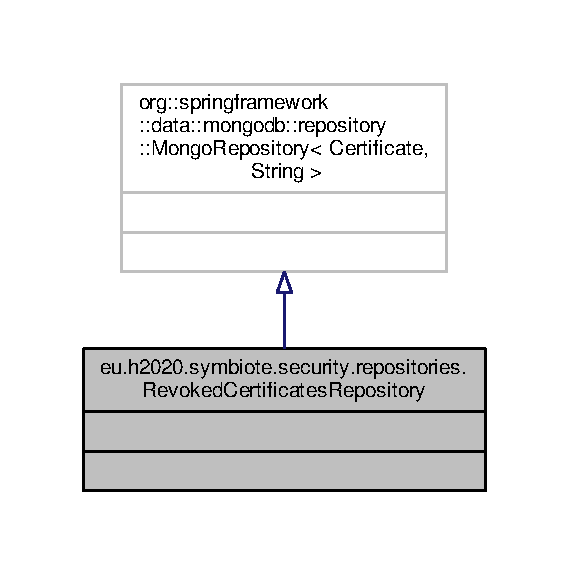
\includegraphics[width=273pt]{interfaceeu_1_1h2020_1_1symbiote_1_1security_1_1repositories_1_1RevokedCertificatesRepository__inherit__graph}
\end{center}
\end{figure}


Collaboration diagram for eu.\+h2020.\+symbiote.\+security.\+repositories.\+Revoked\+Certificates\+Repository\+:
\nopagebreak
\begin{figure}[H]
\begin{center}
\leavevmode
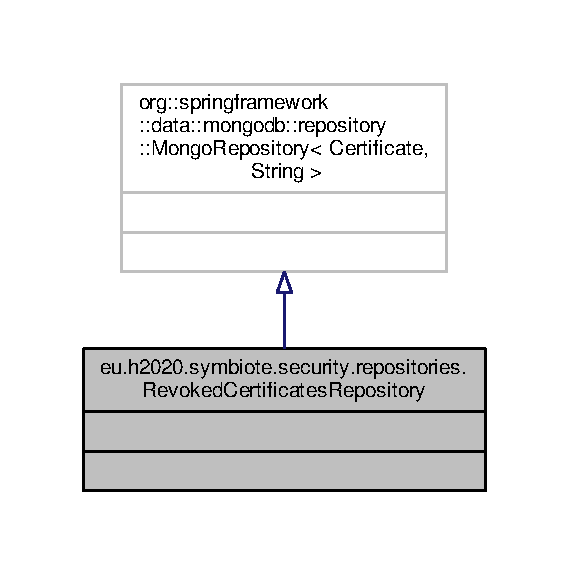
\includegraphics[width=273pt]{interfaceeu_1_1h2020_1_1symbiote_1_1security_1_1repositories_1_1RevokedCertificatesRepository__coll__graph}
\end{center}
\end{figure}


\subsection{Detailed Description}
Spring repository interface definition to be used with Mongo\+DB for operations on revoked certificates.

\begin{DoxyAuthor}{Author}
Daniele Caldarola (C\+N\+IT) 

Nemanja Ignjatov (U\+N\+I\+V\+IE) 
\end{DoxyAuthor}


The documentation for this interface was generated from the following file\+:\begin{DoxyCompactItemize}
\item 
src/main/java/eu/h2020/symbiote/security/repositories/Revoked\+Certificates\+Repository.\+java\end{DoxyCompactItemize}

\hypertarget{classeu_1_1h2020_1_1symbiote_1_1security_1_1rest_1_1TokenController}{}\section{eu.\+h2020.\+symbiote.\+security.\+rest.\+Token\+Controller Class Reference}
\label{classeu_1_1h2020_1_1symbiote_1_1security_1_1rest_1_1TokenController}\index{eu.\+h2020.\+symbiote.\+security.\+rest.\+Token\+Controller@{eu.\+h2020.\+symbiote.\+security.\+rest.\+Token\+Controller}}


Collaboration diagram for eu.\+h2020.\+symbiote.\+security.\+rest.\+Token\+Controller\+:
\nopagebreak
\begin{figure}[H]
\begin{center}
\leavevmode
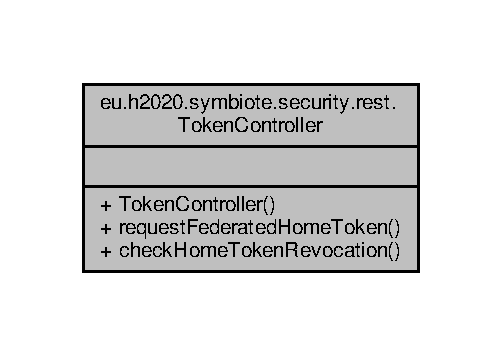
\includegraphics[width=241pt]{classeu_1_1h2020_1_1symbiote_1_1security_1_1rest_1_1TokenController__coll__graph}
\end{center}
\end{figure}
\subsection*{Public Member Functions}
\begin{DoxyCompactItemize}
\item 
{\bfseries Token\+Controller} (\hyperlink{classeu_1_1h2020_1_1symbiote_1_1security_1_1services_1_1TokenService}{Token\+Service} token\+Service, \hyperlink{classeu_1_1h2020_1_1symbiote_1_1security_1_1rest_1_1OtherController}{Other\+Controller} other\+Controller, \hyperlink{classeu_1_1h2020_1_1symbiote_1_1security_1_1commons_1_1RegistrationManager}{Registration\+Manager} registration\+Manager)\hypertarget{classeu_1_1h2020_1_1symbiote_1_1security_1_1rest_1_1TokenController_a874c25b7344d2e3c4a1f31e60cb5470e}{}\label{classeu_1_1h2020_1_1symbiote_1_1security_1_1rest_1_1TokenController_a874c25b7344d2e3c4a1f31e60cb5470e}

\item 
Response\+Entity$<$?$>$ \hyperlink{classeu_1_1h2020_1_1symbiote_1_1security_1_1rest_1_1TokenController_a9147c8773dcc5641313470146020ddbd}{request\+Federated\+Home\+Token} (@Request\+Header(A\+A\+M\+Constants.\+T\+O\+K\+E\+N\+\_\+\+H\+E\+A\+D\+E\+R\+\_\+\+N\+A\+ME) String received\+Token\+String)
\item 
Response\+Entity$<$ Check\+Revocation\+Response $>$ \hyperlink{classeu_1_1h2020_1_1symbiote_1_1security_1_1rest_1_1TokenController_a1393bd5ddb530a43c3021a4cd422bb7a}{check\+Home\+Token\+Revocation} (@Request\+Header(A\+A\+M\+Constants.\+T\+O\+K\+E\+N\+\_\+\+H\+E\+A\+D\+E\+R\+\_\+\+N\+A\+ME) String token\+String)
\end{DoxyCompactItemize}


\subsection{Detailed Description}
Spring controller to handle H\+T\+T\+PS requests related to the R\+E\+S\+Tful web services associated to token objects in Cloud A\+AM component.

\begin{DoxyAuthor}{Author}
Daniele Caldarola (C\+N\+IT) 

Nemanja Ignjatov (U\+N\+I\+V\+IE) 
\end{DoxyAuthor}
\begin{DoxySeeAlso}{See also}
Token\+Service 
\end{DoxySeeAlso}


\subsection{Member Function Documentation}
\index{eu\+::h2020\+::symbiote\+::security\+::rest\+::\+Token\+Controller@{eu\+::h2020\+::symbiote\+::security\+::rest\+::\+Token\+Controller}!check\+Home\+Token\+Revocation@{check\+Home\+Token\+Revocation}}
\index{check\+Home\+Token\+Revocation@{check\+Home\+Token\+Revocation}!eu\+::h2020\+::symbiote\+::security\+::rest\+::\+Token\+Controller@{eu\+::h2020\+::symbiote\+::security\+::rest\+::\+Token\+Controller}}
\subsubsection[{\texorpdfstring{check\+Home\+Token\+Revocation("@Request\+Header(\+A\+A\+M\+Constants.\+T\+O\+K\+E\+N\+\_\+\+H\+E\+A\+D\+E\+R\+\_\+\+N\+A\+M\+E) String token\+String)}{checkHomeTokenRevocation(@RequestHeader(AAMConstants.TOKEN_HEADER_NAME) String tokenString)}}]{\setlength{\rightskip}{0pt plus 5cm}Response\+Entity$<$Check\+Revocation\+Response$>$ eu.\+h2020.\+symbiote.\+security.\+rest.\+Token\+Controller.\+check\+Home\+Token\+Revocation (
\begin{DoxyParamCaption}
\item[{@Request\+Header(A\+A\+M\+Constants.\+T\+O\+K\+E\+N\+\_\+\+H\+E\+A\+D\+E\+R\+\_\+\+N\+A\+ME) String}]{token\+String}
\end{DoxyParamCaption}
)}\hypertarget{classeu_1_1h2020_1_1symbiote_1_1security_1_1rest_1_1TokenController_a1393bd5ddb530a43c3021a4cd422bb7a}{}\label{classeu_1_1h2020_1_1symbiote_1_1security_1_1rest_1_1TokenController_a1393bd5ddb530a43c3021a4cd422bb7a}
L1 Diagrams -\/ check\+\_\+token\+\_\+revocation() T\+O\+DO R3 \index{eu\+::h2020\+::symbiote\+::security\+::rest\+::\+Token\+Controller@{eu\+::h2020\+::symbiote\+::security\+::rest\+::\+Token\+Controller}!request\+Federated\+Home\+Token@{request\+Federated\+Home\+Token}}
\index{request\+Federated\+Home\+Token@{request\+Federated\+Home\+Token}!eu\+::h2020\+::symbiote\+::security\+::rest\+::\+Token\+Controller@{eu\+::h2020\+::symbiote\+::security\+::rest\+::\+Token\+Controller}}
\subsubsection[{\texorpdfstring{request\+Federated\+Home\+Token("@Request\+Header(\+A\+A\+M\+Constants.\+T\+O\+K\+E\+N\+\_\+\+H\+E\+A\+D\+E\+R\+\_\+\+N\+A\+M\+E) String received\+Token\+String)}{requestFederatedHomeToken(@RequestHeader(AAMConstants.TOKEN_HEADER_NAME) String receivedTokenString)}}]{\setlength{\rightskip}{0pt plus 5cm}Response\+Entity$<$?$>$ eu.\+h2020.\+symbiote.\+security.\+rest.\+Token\+Controller.\+request\+Federated\+Home\+Token (
\begin{DoxyParamCaption}
\item[{@Request\+Header(A\+A\+M\+Constants.\+T\+O\+K\+E\+N\+\_\+\+H\+E\+A\+D\+E\+R\+\_\+\+N\+A\+ME) String}]{received\+Token\+String}
\end{DoxyParamCaption}
)}\hypertarget{classeu_1_1h2020_1_1symbiote_1_1security_1_1rest_1_1TokenController_a9147c8773dcc5641313470146020ddbd}{}\label{classeu_1_1h2020_1_1symbiote_1_1security_1_1rest_1_1TokenController_a9147c8773dcc5641313470146020ddbd}
L1 Diagrams -\/ request\+\_\+foreign\+\_\+token() T\+O\+DO R3 

The documentation for this class was generated from the following file\+:\begin{DoxyCompactItemize}
\item 
src/main/java/eu/h2020/symbiote/security/rest/Token\+Controller.\+java\end{DoxyCompactItemize}

\hypertarget{classeu_1_1h2020_1_1symbiote_1_1security_1_1commons_1_1TokenManager}{}\section{eu.\+h2020.\+symbiote.\+security.\+commons.\+Token\+Manager Class Reference}
\label{classeu_1_1h2020_1_1symbiote_1_1security_1_1commons_1_1TokenManager}\index{eu.\+h2020.\+symbiote.\+security.\+commons.\+Token\+Manager@{eu.\+h2020.\+symbiote.\+security.\+commons.\+Token\+Manager}}


Collaboration diagram for eu.\+h2020.\+symbiote.\+security.\+commons.\+Token\+Manager\+:
\nopagebreak
\begin{figure}[H]
\begin{center}
\leavevmode
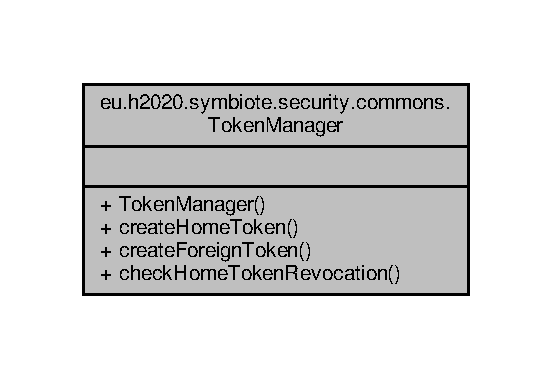
\includegraphics[width=265pt]{classeu_1_1h2020_1_1symbiote_1_1security_1_1commons_1_1TokenManager__coll__graph}
\end{center}
\end{figure}
\subsection*{Public Member Functions}
\begin{DoxyCompactItemize}
\item 
{\bfseries Token\+Manager} (\hyperlink{classeu_1_1h2020_1_1symbiote_1_1security_1_1commons_1_1RegistrationManager}{Registration\+Manager} reg\+Manager, \hyperlink{interfaceeu_1_1h2020_1_1symbiote_1_1security_1_1repositories_1_1PlatformRepository}{Platform\+Repository} platform\+Repository)\hypertarget{classeu_1_1h2020_1_1symbiote_1_1security_1_1commons_1_1TokenManager_a421a9ca8702d476849b8a425dadd9127}{}\label{classeu_1_1h2020_1_1symbiote_1_1security_1_1commons_1_1TokenManager_a421a9ca8702d476849b8a425dadd9127}

\item 
Token \hyperlink{classeu_1_1h2020_1_1symbiote_1_1security_1_1commons_1_1TokenManager_a5f369542764f2b777081e8b071a9a9da}{create\+Home\+Token} (\hyperlink{classeu_1_1h2020_1_1symbiote_1_1security_1_1commons_1_1User}{User} user)  throws J\+W\+T\+Creation\+Exception 
\item 
Token {\bfseries create\+Foreign\+Token} (String foreign\+Token)  throws J\+W\+T\+Creation\+Exception \hypertarget{classeu_1_1h2020_1_1symbiote_1_1security_1_1commons_1_1TokenManager_a40d053bdb0b162a86c5813be3802d722}{}\label{classeu_1_1h2020_1_1symbiote_1_1security_1_1commons_1_1TokenManager_a40d053bdb0b162a86c5813be3802d722}

\item 
Check\+Revocation\+Response {\bfseries check\+Home\+Token\+Revocation} (String token, Token db\+Token)\hypertarget{classeu_1_1h2020_1_1symbiote_1_1security_1_1commons_1_1TokenManager_a169e51ef9a2110174d21baefce1b3309}{}\label{classeu_1_1h2020_1_1symbiote_1_1security_1_1commons_1_1TokenManager_a169e51ef9a2110174d21baefce1b3309}

\end{DoxyCompactItemize}


\subsection{Detailed Description}
Class for managing operations (creation, verification checking, etc.) on tokens in token related service (\hyperlink{}{Token\+Service}).

\begin{DoxyAuthor}{Author}
Daniele Caldarola (C\+N\+IT) 

Nemanja Ignjatov (U\+N\+I\+V\+IE) 

Mikołaj Dobski (P\+S\+NC) 
\end{DoxyAuthor}


\subsection{Member Function Documentation}
\index{eu\+::h2020\+::symbiote\+::security\+::commons\+::\+Token\+Manager@{eu\+::h2020\+::symbiote\+::security\+::commons\+::\+Token\+Manager}!create\+Home\+Token@{create\+Home\+Token}}
\index{create\+Home\+Token@{create\+Home\+Token}!eu\+::h2020\+::symbiote\+::security\+::commons\+::\+Token\+Manager@{eu\+::h2020\+::symbiote\+::security\+::commons\+::\+Token\+Manager}}
\subsubsection[{\texorpdfstring{create\+Home\+Token(\+User user)}{createHomeToken(User user)}}]{\setlength{\rightskip}{0pt plus 5cm}Token eu.\+h2020.\+symbiote.\+security.\+commons.\+Token\+Manager.\+create\+Home\+Token (
\begin{DoxyParamCaption}
\item[{{\bf User}}]{user}
\end{DoxyParamCaption}
) throws J\+W\+T\+Creation\+Exception}\hypertarget{classeu_1_1h2020_1_1symbiote_1_1security_1_1commons_1_1TokenManager_a5f369542764f2b777081e8b071a9a9da}{}\label{classeu_1_1h2020_1_1symbiote_1_1security_1_1commons_1_1TokenManager_a5f369542764f2b777081e8b071a9a9da}

\begin{DoxyParams}{Parameters}
{\em user} & for which to issue to token \\
\hline
\end{DoxyParams}
\begin{DoxyReturn}{Returns}
core or platform token issued for given user 
\end{DoxyReturn}

\begin{DoxyExceptions}{Exceptions}
{\em J\+W\+T\+Creation\+Exception} & on error \\
\hline
\end{DoxyExceptions}


The documentation for this class was generated from the following file\+:\begin{DoxyCompactItemize}
\item 
src/main/java/eu/h2020/symbiote/security/commons/Token\+Manager.\+java\end{DoxyCompactItemize}

\hypertarget{interfaceeu_1_1h2020_1_1symbiote_1_1security_1_1repositories_1_1TokenRepository}{}\section{eu.\+h2020.\+symbiote.\+security.\+repositories.\+Token\+Repository Interface Reference}
\label{interfaceeu_1_1h2020_1_1symbiote_1_1security_1_1repositories_1_1TokenRepository}\index{eu.\+h2020.\+symbiote.\+security.\+repositories.\+Token\+Repository@{eu.\+h2020.\+symbiote.\+security.\+repositories.\+Token\+Repository}}


Inheritance diagram for eu.\+h2020.\+symbiote.\+security.\+repositories.\+Token\+Repository\+:
\nopagebreak
\begin{figure}[H]
\begin{center}
\leavevmode
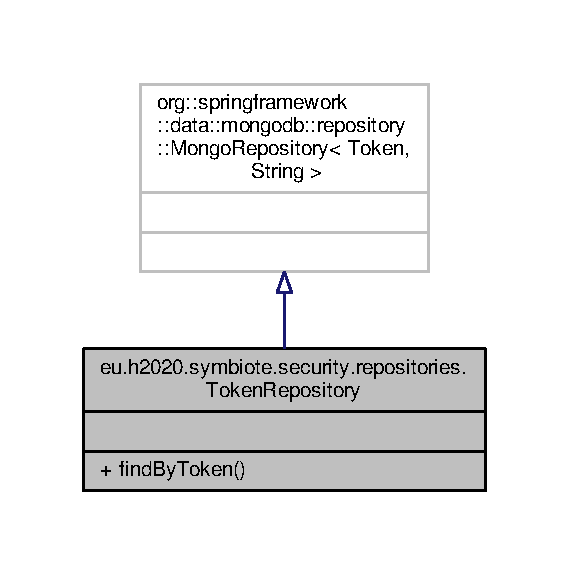
\includegraphics[width=273pt]{interfaceeu_1_1h2020_1_1symbiote_1_1security_1_1repositories_1_1TokenRepository__inherit__graph}
\end{center}
\end{figure}


Collaboration diagram for eu.\+h2020.\+symbiote.\+security.\+repositories.\+Token\+Repository\+:
\nopagebreak
\begin{figure}[H]
\begin{center}
\leavevmode
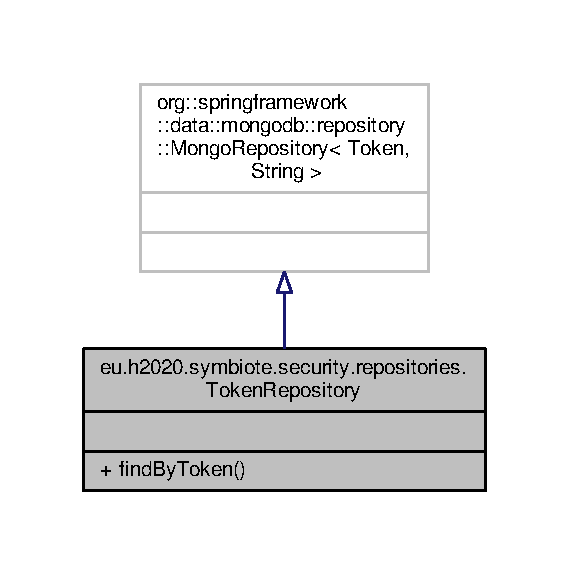
\includegraphics[width=273pt]{interfaceeu_1_1h2020_1_1symbiote_1_1security_1_1repositories_1_1TokenRepository__coll__graph}
\end{center}
\end{figure}
\subsection*{Public Member Functions}
\begin{DoxyCompactItemize}
\item 
Token {\bfseries find\+By\+Token} (String token)\hypertarget{interfaceeu_1_1h2020_1_1symbiote_1_1security_1_1repositories_1_1TokenRepository_a7731062720d5830ffa17bc0d6c3bc70a}{}\label{interfaceeu_1_1h2020_1_1symbiote_1_1security_1_1repositories_1_1TokenRepository_a7731062720d5830ffa17bc0d6c3bc70a}

\end{DoxyCompactItemize}


\subsection{Detailed Description}
Spring repository interface definition to be used with Mongo\+DB for operations on \hyperlink{}{Token} entities.

\begin{DoxyAuthor}{Author}
Daniele Caldarola (C\+N\+IT) 

Nemanja Ignjatov (U\+N\+I\+V\+IE) 
\end{DoxyAuthor}


The documentation for this interface was generated from the following file\+:\begin{DoxyCompactItemize}
\item 
src/main/java/eu/h2020/symbiote/security/repositories/Token\+Repository.\+java\end{DoxyCompactItemize}

\hypertarget{classeu_1_1h2020_1_1symbiote_1_1security_1_1services_1_1TokenService}{}\section{eu.\+h2020.\+symbiote.\+security.\+services.\+Token\+Service Class Reference}
\label{classeu_1_1h2020_1_1symbiote_1_1security_1_1services_1_1TokenService}\index{eu.\+h2020.\+symbiote.\+security.\+services.\+Token\+Service@{eu.\+h2020.\+symbiote.\+security.\+services.\+Token\+Service}}


Collaboration diagram for eu.\+h2020.\+symbiote.\+security.\+services.\+Token\+Service\+:
\nopagebreak
\begin{figure}[H]
\begin{center}
\leavevmode
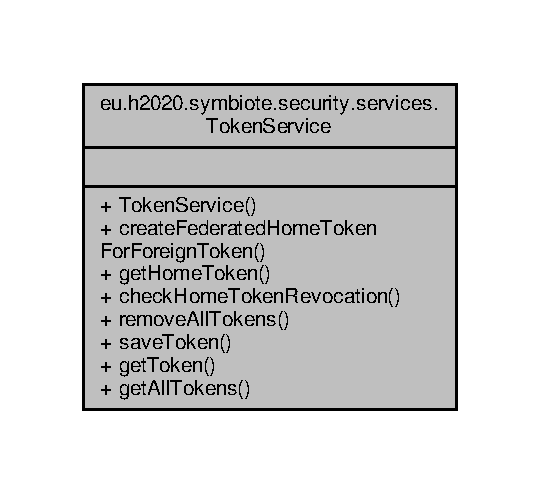
\includegraphics[width=259pt]{classeu_1_1h2020_1_1symbiote_1_1security_1_1services_1_1TokenService__coll__graph}
\end{center}
\end{figure}
\subsection*{Public Member Functions}
\begin{DoxyCompactItemize}
\item 
{\bfseries Token\+Service} (\hyperlink{interfaceeu_1_1h2020_1_1symbiote_1_1security_1_1repositories_1_1TokenRepository}{Token\+Repository} token\+Repository, \hyperlink{classeu_1_1h2020_1_1symbiote_1_1security_1_1commons_1_1TokenManager}{Token\+Manager} token\+Manager)\hypertarget{classeu_1_1h2020_1_1symbiote_1_1security_1_1services_1_1TokenService_ac63dd08a68ce3fb1625b534496856949}{}\label{classeu_1_1h2020_1_1symbiote_1_1security_1_1services_1_1TokenService_ac63dd08a68ce3fb1625b534496856949}

\item 
Token {\bfseries create\+Federated\+Home\+Token\+For\+Foreign\+Token} (String foreign\+Token)  throws J\+W\+T\+Creation\+Exception \hypertarget{classeu_1_1h2020_1_1symbiote_1_1security_1_1services_1_1TokenService_af9f0ff25f06558e38d0d6c301f69c7ab}{}\label{classeu_1_1h2020_1_1symbiote_1_1security_1_1services_1_1TokenService_af9f0ff25f06558e38d0d6c301f69c7ab}

\item 
Token \hyperlink{classeu_1_1h2020_1_1symbiote_1_1security_1_1services_1_1TokenService_a2381d5a63769cff11c281c4d180904cd}{get\+Home\+Token} (\hyperlink{classeu_1_1h2020_1_1symbiote_1_1security_1_1commons_1_1User}{User} user)  throws J\+W\+T\+Creation\+Exception 
\item 
Check\+Revocation\+Response {\bfseries check\+Home\+Token\+Revocation} (String token\+String)\hypertarget{classeu_1_1h2020_1_1symbiote_1_1security_1_1services_1_1TokenService_a86627004cbd20b1eebd16657bba52324}{}\label{classeu_1_1h2020_1_1symbiote_1_1security_1_1services_1_1TokenService_a86627004cbd20b1eebd16657bba52324}

\item 
void {\bfseries remove\+All\+Tokens} ()\hypertarget{classeu_1_1h2020_1_1symbiote_1_1security_1_1services_1_1TokenService_a11455b98f0dd409cead6ce2a9121c741}{}\label{classeu_1_1h2020_1_1symbiote_1_1security_1_1services_1_1TokenService_a11455b98f0dd409cead6ce2a9121c741}

\item 
void {\bfseries save\+Token} (Token token)\hypertarget{classeu_1_1h2020_1_1symbiote_1_1security_1_1services_1_1TokenService_ab7fd9f64e419041cc100dc8900c47188}{}\label{classeu_1_1h2020_1_1symbiote_1_1security_1_1services_1_1TokenService_ab7fd9f64e419041cc100dc8900c47188}

\item 
Token {\bfseries get\+Token} (String jwt)  throws Token\+Validation\+Exception \hypertarget{classeu_1_1h2020_1_1symbiote_1_1security_1_1services_1_1TokenService_aa25ee0afe4d1496a49a94fc4032af544}{}\label{classeu_1_1h2020_1_1symbiote_1_1security_1_1services_1_1TokenService_aa25ee0afe4d1496a49a94fc4032af544}

\item 
List$<$ Token $>$ {\bfseries get\+All\+Tokens} ()\hypertarget{classeu_1_1h2020_1_1symbiote_1_1security_1_1services_1_1TokenService_a3d535c0067c859f568551a88ae8d090e}{}\label{classeu_1_1h2020_1_1symbiote_1_1security_1_1services_1_1TokenService_a3d535c0067c859f568551a88ae8d090e}

\end{DoxyCompactItemize}


\subsection{Detailed Description}
Spring service used to provide token related functionality of the A\+AM.

\begin{DoxyAuthor}{Author}
Daniele Caldarola (C\+N\+IT) 

Nemanja Ignjatov (U\+N\+I\+V\+IE) 
\end{DoxyAuthor}


\subsection{Member Function Documentation}
\index{eu\+::h2020\+::symbiote\+::security\+::services\+::\+Token\+Service@{eu\+::h2020\+::symbiote\+::security\+::services\+::\+Token\+Service}!get\+Home\+Token@{get\+Home\+Token}}
\index{get\+Home\+Token@{get\+Home\+Token}!eu\+::h2020\+::symbiote\+::security\+::services\+::\+Token\+Service@{eu\+::h2020\+::symbiote\+::security\+::services\+::\+Token\+Service}}
\subsubsection[{\texorpdfstring{get\+Home\+Token(\+User user)}{getHomeToken(User user)}}]{\setlength{\rightskip}{0pt plus 5cm}Token eu.\+h2020.\+symbiote.\+security.\+services.\+Token\+Service.\+get\+Home\+Token (
\begin{DoxyParamCaption}
\item[{{\bf User}}]{user}
\end{DoxyParamCaption}
) throws J\+W\+T\+Creation\+Exception}\hypertarget{classeu_1_1h2020_1_1symbiote_1_1security_1_1services_1_1TokenService_a2381d5a63769cff11c281c4d180904cd}{}\label{classeu_1_1h2020_1_1symbiote_1_1security_1_1services_1_1TokenService_a2381d5a63769cff11c281c4d180904cd}

\begin{DoxyParams}{Parameters}
{\em user} & which the token belongs to \\
\hline
\end{DoxyParams}
\begin{DoxyReturn}{Returns}
Generates home token for given user 
\end{DoxyReturn}

\begin{DoxyExceptions}{Exceptions}
{\em J\+W\+T\+Creation\+Exception} & \\
\hline
\end{DoxyExceptions}


The documentation for this class was generated from the following file\+:\begin{DoxyCompactItemize}
\item 
src/main/java/eu/h2020/symbiote/security/services/Token\+Service.\+java\end{DoxyCompactItemize}

\hypertarget{classeu_1_1h2020_1_1symbiote_1_1security_1_1commons_1_1User}{}\section{eu.\+h2020.\+symbiote.\+security.\+commons.\+User Class Reference}
\label{classeu_1_1h2020_1_1symbiote_1_1security_1_1commons_1_1User}\index{eu.\+h2020.\+symbiote.\+security.\+commons.\+User@{eu.\+h2020.\+symbiote.\+security.\+commons.\+User}}


Collaboration diagram for eu.\+h2020.\+symbiote.\+security.\+commons.\+User\+:
\nopagebreak
\begin{figure}[H]
\begin{center}
\leavevmode
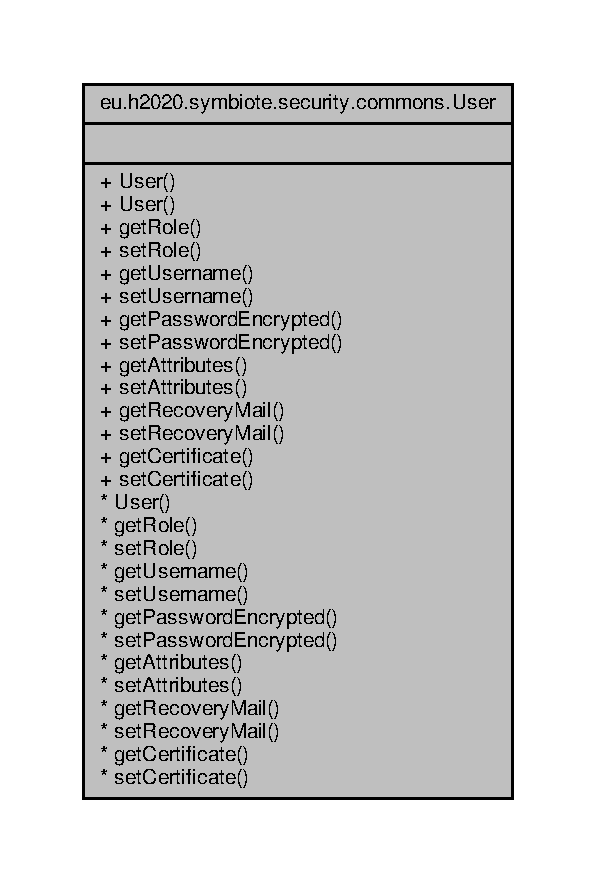
\includegraphics[width=286pt]{classeu_1_1h2020_1_1symbiote_1_1security_1_1commons_1_1User__coll__graph}
\end{center}
\end{figure}
\subsection*{Public Member Functions}
{\bf }\par
\begin{DoxyCompactItemize}
\item 
\hyperlink{classeu_1_1h2020_1_1symbiote_1_1security_1_1commons_1_1User_af6cce37a5c28aacc648c297a6047df0e}{User} (String username, String password\+Encrypted, String recovery\+Mail, Certificate certificate, User\+Role role, List$<$ String $>$ attributes)
\item 
User\+Role {\bfseries get\+Role} ()\hypertarget{classeu_1_1h2020_1_1symbiote_1_1security_1_1commons_1_1User_aaed5c68b3bcef2910de878bf2e93d9c1}{}\label{classeu_1_1h2020_1_1symbiote_1_1security_1_1commons_1_1User_aaed5c68b3bcef2910de878bf2e93d9c1}

\item 
void {\bfseries set\+Role} (User\+Role role)\hypertarget{classeu_1_1h2020_1_1symbiote_1_1security_1_1commons_1_1User_ae41fe3268e2d879af1cdfe09944e8907}{}\label{classeu_1_1h2020_1_1symbiote_1_1security_1_1commons_1_1User_ae41fe3268e2d879af1cdfe09944e8907}

\item 
String {\bfseries get\+Username} ()\hypertarget{classeu_1_1h2020_1_1symbiote_1_1security_1_1commons_1_1User_ad05ea4cfd2aa34788a522c2f92fecd48}{}\label{classeu_1_1h2020_1_1symbiote_1_1security_1_1commons_1_1User_ad05ea4cfd2aa34788a522c2f92fecd48}

\item 
void {\bfseries set\+Username} (String username)\hypertarget{classeu_1_1h2020_1_1symbiote_1_1security_1_1commons_1_1User_a3431410bd8258116f35cecd3226a9f34}{}\label{classeu_1_1h2020_1_1symbiote_1_1security_1_1commons_1_1User_a3431410bd8258116f35cecd3226a9f34}

\item 
String {\bfseries get\+Password\+Encrypted} ()\hypertarget{classeu_1_1h2020_1_1symbiote_1_1security_1_1commons_1_1User_a7a4b0e7eec06d572c46c01c203f6c0d4}{}\label{classeu_1_1h2020_1_1symbiote_1_1security_1_1commons_1_1User_a7a4b0e7eec06d572c46c01c203f6c0d4}

\item 
void {\bfseries set\+Password\+Encrypted} (String password\+Encrypted)\hypertarget{classeu_1_1h2020_1_1symbiote_1_1security_1_1commons_1_1User_ab8eab93ab78698d3e4a2aceafb633b68}{}\label{classeu_1_1h2020_1_1symbiote_1_1security_1_1commons_1_1User_ab8eab93ab78698d3e4a2aceafb633b68}

\item 
List$<$ String $>$ {\bfseries get\+Attributes} ()\hypertarget{classeu_1_1h2020_1_1symbiote_1_1security_1_1commons_1_1User_a9b27b53e587125584372aa44e037fa84}{}\label{classeu_1_1h2020_1_1symbiote_1_1security_1_1commons_1_1User_a9b27b53e587125584372aa44e037fa84}

\item 
void {\bfseries set\+Attributes} (List$<$ String $>$ attributes)\hypertarget{classeu_1_1h2020_1_1symbiote_1_1security_1_1commons_1_1User_a438797ccbef532569a2939c8505dcc35}{}\label{classeu_1_1h2020_1_1symbiote_1_1security_1_1commons_1_1User_a438797ccbef532569a2939c8505dcc35}

\item 
String {\bfseries get\+Recovery\+Mail} ()\hypertarget{classeu_1_1h2020_1_1symbiote_1_1security_1_1commons_1_1User_afd08dcdbfe69b5f899f3b1798b29456f}{}\label{classeu_1_1h2020_1_1symbiote_1_1security_1_1commons_1_1User_afd08dcdbfe69b5f899f3b1798b29456f}

\item 
void {\bfseries set\+Recovery\+Mail} (String recovery\+Mail)\hypertarget{classeu_1_1h2020_1_1symbiote_1_1security_1_1commons_1_1User_a2a33e847fdb6fcc11dd24a6617e649a3}{}\label{classeu_1_1h2020_1_1symbiote_1_1security_1_1commons_1_1User_a2a33e847fdb6fcc11dd24a6617e649a3}

\item 
Certificate {\bfseries get\+Certificate} ()\hypertarget{classeu_1_1h2020_1_1symbiote_1_1security_1_1commons_1_1User_ab4f8e1351a6895d2dfa70a4e9e6b446b}{}\label{classeu_1_1h2020_1_1symbiote_1_1security_1_1commons_1_1User_ab4f8e1351a6895d2dfa70a4e9e6b446b}

\item 
void {\bfseries set\+Certificate} (Certificate certificate)\hypertarget{classeu_1_1h2020_1_1symbiote_1_1security_1_1commons_1_1User_a03534851356555a495f62528995832e4}{}\label{classeu_1_1h2020_1_1symbiote_1_1security_1_1commons_1_1User_a03534851356555a495f62528995832e4}

\end{DoxyCompactItemize}



\subsection{Detailed Description}
Class for symb\+Io\+Te\textquotesingle{}s user entity -- an Application or Platform\+Owner

\begin{DoxyAuthor}{Author}
Daniele Caldarola (C\+N\+IT) 

Nemanja Ignjatov (U\+N\+I\+V\+IE) 

Mikołaj Dobski (P\+S\+NC) 
\end{DoxyAuthor}


\subsection{Constructor \& Destructor Documentation}
\index{eu\+::h2020\+::symbiote\+::security\+::commons\+::\+User@{eu\+::h2020\+::symbiote\+::security\+::commons\+::\+User}!User@{User}}
\index{User@{User}!eu\+::h2020\+::symbiote\+::security\+::commons\+::\+User@{eu\+::h2020\+::symbiote\+::security\+::commons\+::\+User}}
\subsubsection[{\texorpdfstring{User(\+String username, String password\+Encrypted, String recovery\+Mail, Certificate certificate, User\+Role role, List$<$ String $>$ attributes)}{User(String username, String passwordEncrypted, String recoveryMail, Certificate certificate, UserRole role, List< String > attributes)}}]{\setlength{\rightskip}{0pt plus 5cm}eu.\+h2020.\+symbiote.\+security.\+commons.\+User.\+User (
\begin{DoxyParamCaption}
\item[{String}]{username, }
\item[{String}]{password\+Encrypted, }
\item[{String}]{recovery\+Mail, }
\item[{Certificate}]{certificate, }
\item[{User\+Role}]{role, }
\item[{List$<$ String $>$}]{attributes}
\end{DoxyParamCaption}
)}\hypertarget{classeu_1_1h2020_1_1symbiote_1_1security_1_1commons_1_1User_af6cce37a5c28aacc648c297a6047df0e}{}\label{classeu_1_1h2020_1_1symbiote_1_1security_1_1commons_1_1User_af6cce37a5c28aacc648c297a6047df0e}
Used to create a new user entity


\begin{DoxyParams}{Parameters}
{\em username} & selected username \\
\hline
{\em password\+Encrypted} & encrypted password for authentication \\
\hline
{\em recovery\+Mail} & for password reset/recovery purposes \\
\hline
{\em certificate} & user\textquotesingle{}s public certificate \\
\hline
{\em role} & user\textquotesingle{}s role in symb\+Io\+Te ecosystem, see\hyperlink{}{\}  attributes used to assign in registration phase application-\/unique attributes }\\
\hline
\end{DoxyParams}


The documentation for this class was generated from the following file\+:\begin{DoxyCompactItemize}
\item 
src/main/java/eu/h2020/symbiote/security/commons/User.\+java\end{DoxyCompactItemize}

\hypertarget{classeu_1_1h2020_1_1symbiote_1_1security_1_1services_1_1UserRegistrationService}{}\section{eu.\+h2020.\+symbiote.\+security.\+services.\+User\+Registration\+Service Class Reference}
\label{classeu_1_1h2020_1_1symbiote_1_1security_1_1services_1_1UserRegistrationService}\index{eu.\+h2020.\+symbiote.\+security.\+services.\+User\+Registration\+Service@{eu.\+h2020.\+symbiote.\+security.\+services.\+User\+Registration\+Service}}


Collaboration diagram for eu.\+h2020.\+symbiote.\+security.\+services.\+User\+Registration\+Service\+:
\nopagebreak
\begin{figure}[H]
\begin{center}
\leavevmode
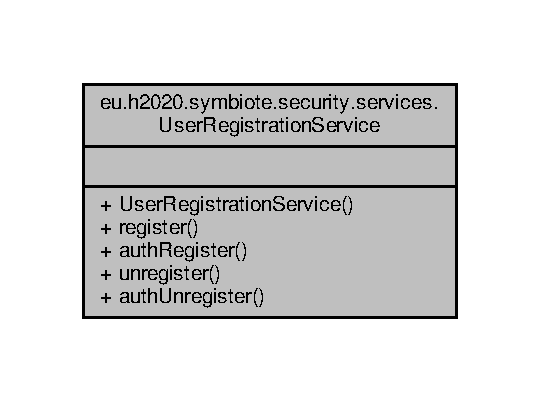
\includegraphics[width=259pt]{classeu_1_1h2020_1_1symbiote_1_1security_1_1services_1_1UserRegistrationService__coll__graph}
\end{center}
\end{figure}
\subsection*{Public Member Functions}
\begin{DoxyCompactItemize}
\item 
{\bfseries User\+Registration\+Service} (\hyperlink{interfaceeu_1_1h2020_1_1symbiote_1_1security_1_1repositories_1_1UserRepository}{User\+Repository} user\+Repository, \hyperlink{interfaceeu_1_1h2020_1_1symbiote_1_1security_1_1repositories_1_1RevokedCertificatesRepository}{Revoked\+Certificates\+Repository} revoked\+Certificates\+Repository, \hyperlink{classeu_1_1h2020_1_1symbiote_1_1security_1_1commons_1_1RegistrationManager}{Registration\+Manager} registration\+Manager, Password\+Encoder password\+Encoder)\hypertarget{classeu_1_1h2020_1_1symbiote_1_1security_1_1services_1_1UserRegistrationService_a608a1985221a57abe21f72f8f3d1c971}{}\label{classeu_1_1h2020_1_1symbiote_1_1security_1_1services_1_1UserRegistrationService_a608a1985221a57abe21f72f8f3d1c971}

\item 
User\+Registration\+Response {\bfseries register} (User\+Registration\+Request user\+Registration\+Request)  throws A\+A\+M\+Exception \hypertarget{classeu_1_1h2020_1_1symbiote_1_1security_1_1services_1_1UserRegistrationService_aff366e7d6fd800cb052ab1b8382d65db}{}\label{classeu_1_1h2020_1_1symbiote_1_1security_1_1services_1_1UserRegistrationService_aff366e7d6fd800cb052ab1b8382d65db}

\item 
User\+Registration\+Response {\bfseries auth\+Register} (User\+Registration\+Request request)  throws A\+A\+M\+Exception \hypertarget{classeu_1_1h2020_1_1symbiote_1_1security_1_1services_1_1UserRegistrationService_acf0d26da645d54dab064cc6dd1bdeab3}{}\label{classeu_1_1h2020_1_1symbiote_1_1security_1_1services_1_1UserRegistrationService_acf0d26da645d54dab064cc6dd1bdeab3}

\item 
void {\bfseries unregister} (String username)  throws A\+A\+M\+Exception \hypertarget{classeu_1_1h2020_1_1symbiote_1_1security_1_1services_1_1UserRegistrationService_a0c210b7334d284674a19aed79a32d4aa}{}\label{classeu_1_1h2020_1_1symbiote_1_1security_1_1services_1_1UserRegistrationService_a0c210b7334d284674a19aed79a32d4aa}

\item 
void {\bfseries auth\+Unregister} (User\+Registration\+Request request)  throws A\+A\+M\+Exception \hypertarget{classeu_1_1h2020_1_1symbiote_1_1security_1_1services_1_1UserRegistrationService_ac107bca35e067f27926f563f865e5386}{}\label{classeu_1_1h2020_1_1symbiote_1_1security_1_1services_1_1UserRegistrationService_ac107bca35e067f27926f563f865e5386}

\end{DoxyCompactItemize}


\subsection{Detailed Description}
Spring service used to register users in the A\+AM repository.

\begin{DoxyAuthor}{Author}
Daniele Caldarola (C\+N\+IT) 

Nemanja Ignjatov (U\+N\+I\+V\+IE) 

Mikołaj Dobski (P\+S\+NC) 
\end{DoxyAuthor}


The documentation for this class was generated from the following file\+:\begin{DoxyCompactItemize}
\item 
src/main/java/eu/h2020/symbiote/security/services/User\+Registration\+Service.\+java\end{DoxyCompactItemize}

\hypertarget{interfaceeu_1_1h2020_1_1symbiote_1_1security_1_1repositories_1_1UserRepository}{}\section{eu.\+h2020.\+symbiote.\+security.\+repositories.\+User\+Repository Interface Reference}
\label{interfaceeu_1_1h2020_1_1symbiote_1_1security_1_1repositories_1_1UserRepository}\index{eu.\+h2020.\+symbiote.\+security.\+repositories.\+User\+Repository@{eu.\+h2020.\+symbiote.\+security.\+repositories.\+User\+Repository}}


Inheritance diagram for eu.\+h2020.\+symbiote.\+security.\+repositories.\+User\+Repository\+:
\nopagebreak
\begin{figure}[H]
\begin{center}
\leavevmode
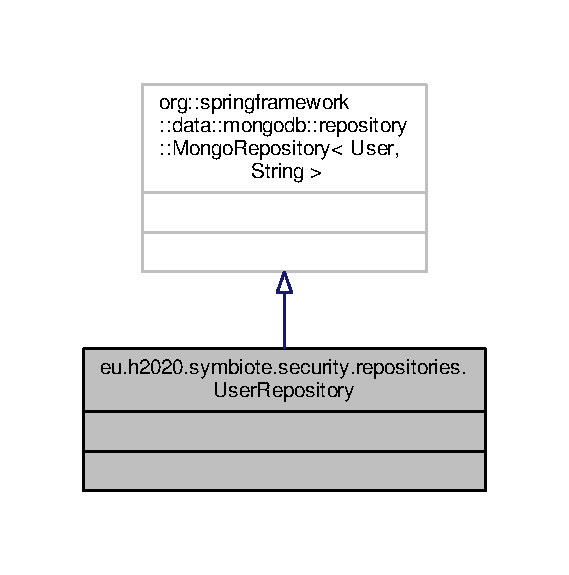
\includegraphics[width=273pt]{interfaceeu_1_1h2020_1_1symbiote_1_1security_1_1repositories_1_1UserRepository__inherit__graph}
\end{center}
\end{figure}


Collaboration diagram for eu.\+h2020.\+symbiote.\+security.\+repositories.\+User\+Repository\+:
\nopagebreak
\begin{figure}[H]
\begin{center}
\leavevmode
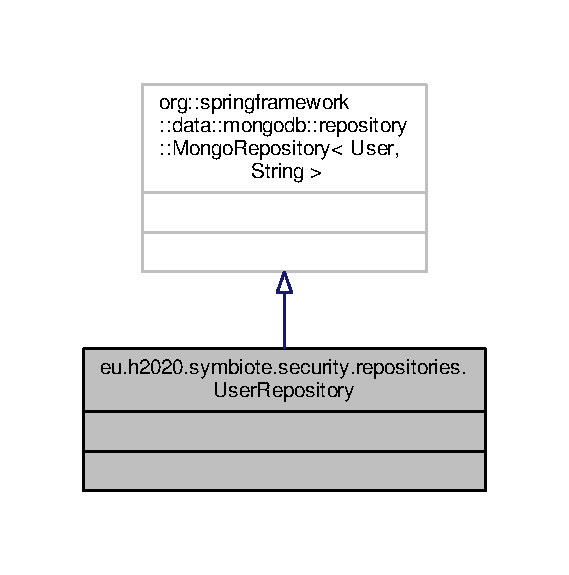
\includegraphics[width=273pt]{interfaceeu_1_1h2020_1_1symbiote_1_1security_1_1repositories_1_1UserRepository__coll__graph}
\end{center}
\end{figure}


\subsection{Detailed Description}
Spring repository interface definition to be used with Mongo\+DB for operations on \hyperlink{}{User} entities.

\begin{DoxyAuthor}{Author}
Daniele Caldarola (C\+N\+IT) 

Nemanja Ignjatov (U\+N\+I\+V\+IE) 
\end{DoxyAuthor}


The documentation for this interface was generated from the following file\+:\begin{DoxyCompactItemize}
\item 
src/main/java/eu/h2020/symbiote/security/repositories/User\+Repository.\+java\end{DoxyCompactItemize}

\hypertarget{classeu_1_1h2020_1_1symbiote_1_1security_1_1commons_1_1VirtualFile}{}\section{eu.\+h2020.\+symbiote.\+security.\+commons.\+Virtual\+File Class Reference}
\label{classeu_1_1h2020_1_1symbiote_1_1security_1_1commons_1_1VirtualFile}\index{eu.\+h2020.\+symbiote.\+security.\+commons.\+Virtual\+File@{eu.\+h2020.\+symbiote.\+security.\+commons.\+Virtual\+File}}


Collaboration diagram for eu.\+h2020.\+symbiote.\+security.\+commons.\+Virtual\+File\+:
\nopagebreak
\begin{figure}[H]
\begin{center}
\leavevmode
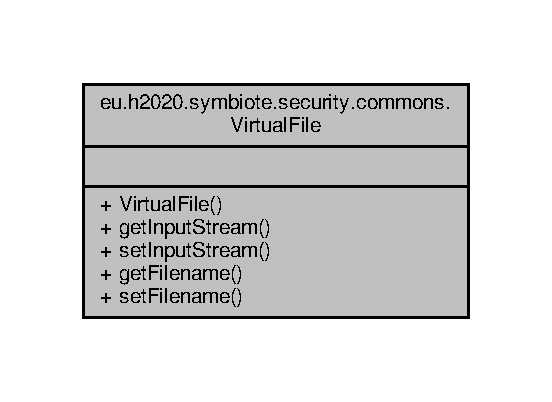
\includegraphics[width=265pt]{classeu_1_1h2020_1_1symbiote_1_1security_1_1commons_1_1VirtualFile__coll__graph}
\end{center}
\end{figure}
\subsection*{Public Member Functions}
\begin{DoxyCompactItemize}
\item 
{\bfseries Virtual\+File} (Input\+Stream input\+Stream, String filename)\hypertarget{classeu_1_1h2020_1_1symbiote_1_1security_1_1commons_1_1VirtualFile_a4f3c734a8179a11e127ae2ed1ff93843}{}\label{classeu_1_1h2020_1_1symbiote_1_1security_1_1commons_1_1VirtualFile_a4f3c734a8179a11e127ae2ed1ff93843}

\item 
Input\+Stream {\bfseries get\+Input\+Stream} ()\hypertarget{classeu_1_1h2020_1_1symbiote_1_1security_1_1commons_1_1VirtualFile_ab8e51b0bafbe996f641576d91d4ce2a8}{}\label{classeu_1_1h2020_1_1symbiote_1_1security_1_1commons_1_1VirtualFile_ab8e51b0bafbe996f641576d91d4ce2a8}

\item 
void {\bfseries set\+Input\+Stream} (Input\+Stream input\+Stream)\hypertarget{classeu_1_1h2020_1_1symbiote_1_1security_1_1commons_1_1VirtualFile_a176717db92b70b7b611cf3e93b2dfe49}{}\label{classeu_1_1h2020_1_1symbiote_1_1security_1_1commons_1_1VirtualFile_a176717db92b70b7b611cf3e93b2dfe49}

\item 
String {\bfseries get\+Filename} ()\hypertarget{classeu_1_1h2020_1_1symbiote_1_1security_1_1commons_1_1VirtualFile_a6d4312b65690866f053b14802d5b4d91}{}\label{classeu_1_1h2020_1_1symbiote_1_1security_1_1commons_1_1VirtualFile_a6d4312b65690866f053b14802d5b4d91}

\item 
void {\bfseries set\+Filename} (String filename)\hypertarget{classeu_1_1h2020_1_1symbiote_1_1security_1_1commons_1_1VirtualFile_a2f094abc06a506737d6534f4d2f051d6}{}\label{classeu_1_1h2020_1_1symbiote_1_1security_1_1commons_1_1VirtualFile_a2f094abc06a506737d6534f4d2f051d6}

\end{DoxyCompactItemize}


The documentation for this class was generated from the following file\+:\begin{DoxyCompactItemize}
\item 
src/main/java/eu/h2020/symbiote/security/commons/Virtual\+File.\+java\end{DoxyCompactItemize}

\hypertarget{classeu_1_1h2020_1_1symbiote_1_1security_1_1services_1_1ZipService}{}\section{eu.\+h2020.\+symbiote.\+security.\+services.\+Zip\+Service Class Reference}
\label{classeu_1_1h2020_1_1symbiote_1_1security_1_1services_1_1ZipService}\index{eu.\+h2020.\+symbiote.\+security.\+services.\+Zip\+Service@{eu.\+h2020.\+symbiote.\+security.\+services.\+Zip\+Service}}


Collaboration diagram for eu.\+h2020.\+symbiote.\+security.\+services.\+Zip\+Service\+:
\nopagebreak
\begin{figure}[H]
\begin{center}
\leavevmode
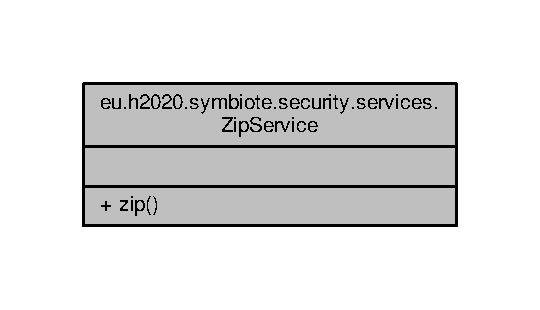
\includegraphics[width=259pt]{classeu_1_1h2020_1_1symbiote_1_1security_1_1services_1_1ZipService__coll__graph}
\end{center}
\end{figure}
\subsection*{Public Member Functions}
\begin{DoxyCompactItemize}
\item 
void {\bfseries zip} (List$<$ \hyperlink{classeu_1_1h2020_1_1symbiote_1_1security_1_1commons_1_1VirtualFile}{Virtual\+File} $>$ virtual\+Files, Output\+Stream output\+Stream)  throws Zip\+Exception, I\+O\+Exception \hypertarget{classeu_1_1h2020_1_1symbiote_1_1security_1_1services_1_1ZipService_ad1a60a49166495e1ee4524f5102edbf7}{}\label{classeu_1_1h2020_1_1symbiote_1_1security_1_1services_1_1ZipService_ad1a60a49166495e1ee4524f5102edbf7}

\end{DoxyCompactItemize}


\subsection{Detailed Description}
Spring service to provide zip output streams.

\begin{DoxyAuthor}{Author}
Daniele Caldarola (C\+N\+IT) 

Nemanja Ignjatov (U\+N\+I\+V\+IE) 
\end{DoxyAuthor}


The documentation for this class was generated from the following file\+:\begin{DoxyCompactItemize}
\item 
src/main/java/eu/h2020/symbiote/security/services/Zip\+Service.\+java\end{DoxyCompactItemize}

%--- End generated contents ---

% Index
\backmatter
\newpage
\phantomsection
\clearemptydoublepage
\addcontentsline{toc}{chapter}{Index}
\printindex

\end{document}
